\documentclass[11pt,a4paper,DIVcalc,BCOR8mm,titlepage,twoside]{scrartcl}

%\usepackage[parfill]{parskip}    % Activate to begin paragraphs with an empty line rather than an indent
\usepackage{german}
\usepackage{amsmath}
\usepackage{amsfonts}
\usepackage{amssymb}
\usepackage{graphicx}
\usepackage{algorithmic}
\usepackage{natbib}
\bibpunct{(}{)}{;}{a}{}{,} % to follow the A&A style

\begin{document}
	\titlehead{Christian--Albrechts--Universit"at zu Kiel\\ Institut f"ur Theoretische Physik und Astrophysik}
	\subject{Diplomarbeit}
	\title{L"osung des Strahlungstransportproblems in Pfadintegralform mit effizienten Monte--Carlo--Verfahren}
	\author{vorgelegt von Thies Heidecke\\(theidecke@astrophysik.uni-kiel.de)}
	\publishers{betreut durch Prof. Sebastian Wolf}
	\date{Version vom \today}
	\maketitle
	% standard-titelblatt verf"ugbar?

	\tableofcontents
	\vfill
	\pagebreak
	
	\newcommand{\location}[1]{\mathbf{#1}}
	\newcommand{\scatter}[1]{\overset{#1}{\leftrightsquigarrow}}
	\newcommand{\normalized}[1]{\frac{#1}{||#1||}}
	
		\chapter{Einleitung}
	\section{Motivation}
	Menschen sind schon immer fasziniert von der Frage nach ihrer eigenen Herkunft und des Universums in dem sie Leben. Eine Facette dieser Frage ist der Wunsch, ein besseres Verständnis des kosmischen Zyklus von der Entstehung und dem Vergehen von Sternen zu erlangen. Dieses Thema ist insbesondere deshalb interessant, weil mit ihm die Entstehung von Planetensystemen verknüpft ist und es somit unsere eigene Herkunft berührt.
	
	In der Astrophysik lassen sich dabei zwei Wege einschlagen um sich diesem Ver\-ständ\-nis zu nähern. Der eine Weg führt über die Beobachtung der Sternentstehungsgebiete am Himmel, in denen nebeneinander verschiedene Entwicklungsstadien der Sternentstehung von Molekülwolken über Globulen, junge stellare Objekte (YSOs) mit protoplanetarer Scheibe, Vorhauptreihensterne und schließlich Hauptreihensterne beobachtet werden können.
	%\begin{wrapfigure}{l}{0.382\textwidth}
	%	\centering
	%	\vspace{-1em}
	%	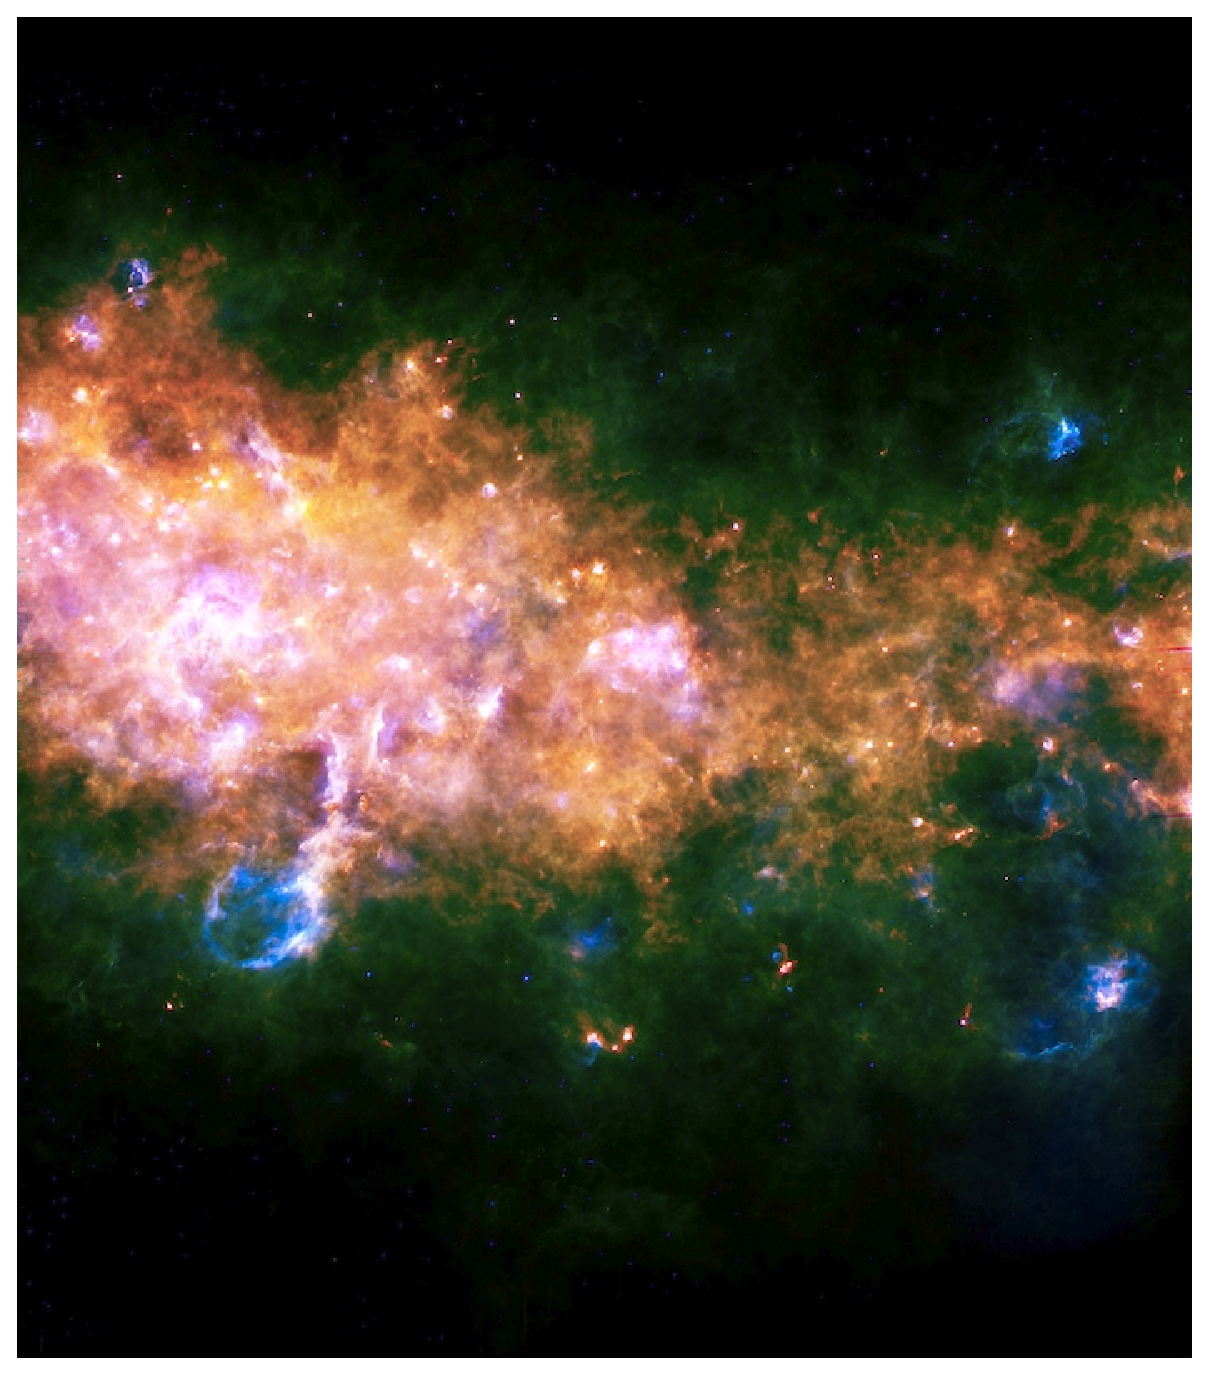
\includegraphics[width=0.382\textwidth]{Stellar_Gestation_and_Birth_in_the_Milky_Way.eps}
	%	\caption{Stern\-ent\-steh\-ungs\-ge\-biet im Ad\-ler\-ne\-bel. Auf\-ge\-nom\-men mit Her\-schel bei 70, 160 und 250$\mu$m im Dezember 2009.}
		% ($18^\text{h}46^\text{m}5.22^\text{s}$ / $+2^\circ 36'32.88"$)
	%	\vspace{-2em}
	%	\label{fig:starformingregion}
	%\end{wrapfigure}
	Auf den verschiedenen Beobachtungen lassen sich empirisch Theorien der Stern- und Planetenentstehung gründen. Der andere Weg führt von etablierten allgemeinen Theorien ausgehend über mathematische Herleitungen oder ``first--principles''--Simulationen zu Vorhersagen oder dem Nachvollzug der verschiedenen Phasen der Stern- und Planetenentstehung. Beide Wege sind nicht unabhängig voneinander sondern bilden vielmehr Abschnitte auf einem spiralförmigen Weg auf dem sich Empirie und Theorie abwechseln und durch Induktion und Deduktion gegenseitig eine bessere Ausgangslage schaffen.
	
	Im Bereich protoplanetarer Scheiben bildet Strahlungstransport den Teil der Theorie, der Vorhersagen über das Verhalten von Licht in einer vorgegebenen Anordnung von Materie macht. Strahlungstransport ist im Bereich protostellarer Scheiben somit einerseits wichtig für ein vollständiges Modell ihres Aufbaus, und andererseits wichtig, um ihr Aussehen vorherzusagen. Eine Simulation des Strahlungstransports erlaubt den Vergleich von Bildern aus Scheibenmodellen und mithilfe von Teleskopen aufgenommener Bilder und stellt somit das direkte Bindeglied zwischen Theorie und Beobachtung dar.
	
	Wir leben dabei in einer spannenden Zeit, in der die aktuelle und kommende Generation von Großteleskopen auf der Erde und im Weltraum detailreichere Daten von protostellaren Scheiben aufnehmen als je zuvor. Dies stellt auch höhere Anforderungen an Strahlungstransportsimulationen, von denen feinere und genauere Bilder und Spektren gebraucht werden um beim Vergleich mit Beobachtungsdaten von Nutzen zu sein.
	
	Dabei stellt sich häufig nicht das Problem, das Aussehen einer vorgegebenen Scheibenkonfiguration zu simulieren, sondern das inverse Problem, aus gegebenen Beobachtungsdaten unter physikalischen Nebenbedingungen die wahrscheinlichste Materieanordnung zu finden um die Beobachtung zu erklären. Das direkte Lösen dieses Problems ist i.A. nicht möglich. Daher ist der praktisch gegangene Ausweg das mehr oder weniger intelligente Raten von möglichst passenden Scheibenkonfigurationen, die nach einer Strahlungstransportsimulation mit den Beobachtungsdaten verglichen werden können. In dieser Situation ist eine effiziente Simulation umso nützlicher und u.U. entscheidend für den Unterschied zwischen dem Raten eines spezifischen Modells aufgrund einiger weniger Modellrechnungen und einer abdeckenden, statistisch signifikanten Schätzung der Modellparameter.
	
	Daher sollen in dieser Arbeit neue Ansätze zur effizienten Lösung des Strahlungstransportproblems vorgestellt, erprobt und diskutiert werden.
	
	\section{Ziele der Arbeit}
	In dieser Arbeit wird eine Pfadintegraldarstellung der Lösung des Strahlungstransportgleichung hergeleitet, sowie dessen Nutzen für Monte--Carlo--Verfahren zur Lösung des Strahlungstransportproblems theoretisch und praktisch in Form eines Computerprogrammes gezeigt.
	
	\section{Übersicht}
	Wir fangen in Kapitel 2 mit einer Einführung des Strahlungstransportproblems über ein allgemeines Teilchentransportproblem an, welches wir anschließend durch Spezialisierung der Teilchen auf Photonen auf die klassische Strahlungstransportgleichung zurückführen. Außerdem stellen wir einen allgemeinen Formalismus für Messungen des Strahlungsfeldes vor.
	
	In Kapitel 3 überführen wir die klassische Strahlungstransportgleichung über den Umweg einer Integraldarstellung in eine Operatorform, in der das Problem anschaulich und formal leicht lösbar ist. Die gewonnene Lösung stellen wir dann als Integral über den Raum aller möglichen Lichtpfade dar.
	
	In Kapitel 4 beschäftigen wir uns mit dem Problem der numerischen Integration und den Vor- und Nachteilen der Monte--Carlo--Integration im Vergleich zu klassischen numerischen Quadraturverfahren.
	
	In Kapitel 5 stellen wir ein weiteres Monte--Carlo--Verfahren vor, mit dem sich aus beliebigen statistischen Verteilungen Stichproben erzeugen lassen und erklären, wozu dies im Zusammenhang mit der Lösung des Strahlungstransportproblems nützlich ist.
	
	In Kapitel 6 führen wir die bis dahin behandelten Themen Strahlungstransport und Monte--Carlo--Verfahren zusammen. Wir zeigen, wie sich die in Kapitel 3 hergeleitete Pfadintegrallösung des Strahlungstransportproblems als Integrationsproblem darstellen lässt, auf die unsere Monte--Carlo--Integrationsverfahren aus Kapitel 4 direkt anwendbar sind. Ergänzend dazu stellen wir Methoden vor, um die Konvergenz der Integration durch eine gehäuftere Berücksichtigung der für den Strahlungstransport wesentlichen Pfade zu verbessern.
	
	In Kapitel 7 stellen wir das Programm \pirate vor, in dem viele der vorgestellten Ideen implementiert sind.
	
	In Kapitel 8 vergleichen wir dann die Ergebnisse und die Geschwindigkeit von \pirate mit dem Referenzprogramm \texttt{MC3D}.
	
	Schließlich fassen wir in Kapitel 9 die Arbeit zusammen und geben einen Ausblick, wie die vorgestellten Ideen und das Programm \pirate weiterentwickelt und eingesetzt werden können.
	
	\vfill
	\pagebreak
	\section{Nomenklatur}\label{subsec:nomenklatur}
	Im folgenden Text werden die in Tabelle \ref{tab:nomenklatur} angegebenen Schreibweisen benutzt.

	\begin{table}
		\caption{Nomenklatur}
		\begin{center}
		\begin{tabular}{rll}
			Schreibweise & Bedeutung & Einheit \\
			\hline
			$\kappa(\location{r})$ & Volumenabsorptionsquerschnitt am Ort $\location{r}$& $\left[\text{m}^2/\text{m}^3\right]$ \\
			$\sigma(\location{r})$ & Volumenstreuquerschnitt am Ort $\location{r}$ & $\left[\text{m}^2/\text{m}^3\right]$ \\
			$\xi(\location{r})$ & Volumenextinktionsquerschnitt am Ort $\location{r}$ & $\left[\text{m}^2/\text{m}^3\right]$ \\
			$\varepsilon(\location{r},\omega)$ & Volumenemissivität am Ort $\location{r}$ in Richtung $\omega$ & $\left[\text{W}/(\text{m}^3\,\text{sr})\right]$ \\
			$I(\location{r},\omega)$ & Intensität am Ort $\location{r}$ in Richtung $\omega$& $\left[\text{W}/(\text{m}^2\,\text{sr})\right]$ \\
			$W(\location{r},\omega)$ & Sensitivität am Ort $\location{r}$ in Richtung $\omega$ & $\left[(\text{m}^2\,\text{sr})/\text{W}\right]$ \\
			$k(\location{r},\omega',\omega)$ & Phasenfunktion am Ort $\location{r}$ für ein Teilchen, & $\left[1/\text{sr}\right]$ \\
				&das sich vor der Streuung in Richtung $\omega'$&\\
				&und nach der Streuung in Richtung $\omega$ bewegt& \\
			$\tau(\location{r}_i,\location{r}_j)$ & Optische Tiefe zwischen $\location{r}_i$ und $\location{r}_j$ & \\
			$\varepsilon_{(i,j)}$ & Emissivität am Ort $\location{r}_i$ in Richtung $\normalized{\location{r}_j-\location{r}_i}$ & \\
			$W_{(i,j)}$ & Sensitivität am Ort $\location{r}_j$ für Strahlung in Richtung $\normalized{\location{r}_j-\location{r}_i}$ & \\
			$\scatter{i}$ & Produkt aus Volumenstreuquerschnitt und&\\
			  & Streuphasenfunktion am Ort $\location{r}_i$ für ein aus Richtung $\location{r}_{i-1}$&\\ 
				&kommendes und in Richtung $\location{r}_{i+1}$ gestreutes Teilchen&\\
				&(äquivalent zu $\sigma(\location{r}_i)k(\location{r}_i,\normalized{\location{r}_i-\location{r}_{i-1}},\normalized{\location{r}_{i+1}-\location{r}_i})$)& \\
			$\propagate{i}{j}$ & Produkt aus Abschwächungsfaktor aufgrund optischer Tiefe&\\
			  &und geometrischem Verdünnungsfaktor zwischen $\location{r}_i$ und $\location{r}_{j}$&\\ 
				&(äquivalent zu $\frac{e^{-\tau(\location{r}_{i},\location{r}_j)}}{\|\location{r}_j-\location{r}_{i}\|^2}$)& \\
			
		\end{tabular}
		\end{center}
		\label{tab:nomenklatur}
	\end{table}

		\chapter{Das Strahlungstransportproblem}
	\label{sec:radiative_transfer}
	
	Das Verhalten von Licht lässt sich (nach heutigem wissenschaftlichen Stand) durch die {\em Quantenelektrodynamik}\footnote{s. z.B. \citet{Feynman:1990p11684}} in allen Details vollständig beschreiben. Es beinhaltet Phänomene wie Dispersion, Brechung, Interferenz, Photon--Photon--Interaktion, etc. Diese Effekte sind häufig dann am bedeutendsten, wenn die Ausmaße der betrachteten Objekte von der Größenordnung der Wellenlänge des Lichtes sind. Auf der anderen Seite beschreibt die {\em geometrische Optik} die rein makroskopische lineare Ausbreitung großer Mengen von Photonen ohne Wellen--Phänomene zu berücksichtigen.
	
	Beim Strahlungstransportproblem (STP) sind wir an einer {\em phänomenologischen} Beschreibung interessiert. Das heißt wir wollen die Intensität des Lichts modellieren, die in typischen Anwendungen durch optische Instrumente (Auge, Teleskope mit Photoplatten/CCD--Chips) gemessen werden kann. Dies bedeutet, dass wir hauptsächlich eine geometrische Beschreibung des Lichts in Form eines Teilchentransportproblems ansetzen aber quantenmechanische Effekte wie Photonen--Streuung in erster Ordnung lokal mitberücksichtigen (z.B. in Form einer Streuphasenfunktion).
	
	Die folgende Darstellung und Herleitung orientiert sich an \citep{Arvo:1993p9035}.
	
	\section{Das Strahlungstransportproblem als Teilchentransportproblem}
	Um Strahlungstransport als Teilchentransportproblem behandeln zu können, müssen folgende Bedingungen erfüllt sein:
	\begin{itemize}
		\item{Die Teilchen müssen so klein und zahlreich sein, dass ihre statistische Verteilung als kontinuierlich angesehen werden kann}
		\item{Zu jedem Zeitpunkt lässt sich ein Teilchen komplett durch Position, Impuls und eventuelle interne Zustände (wie Polarisation, Frequenz, Ladung, Spin, etc.) charakterisieren}
	\end{itemize}
	Diese Annahmen sind für Photonen und die uns interessierenden räumlichen Entfernungen erfüllt.
	Darüber hinausgehend machen wir im Rahmen dieser Arbeit folgende Annahmen:
	\begin{itemize}
		\item{Die Materialeigenschaften ändern sich bei Variation des Ortes in der Größenordnung der Wellenlänge nur wenig}
		\item{Das Strahlungsintensitätsfeld ist stationär, d.h. innerhalb der typischen Zeiten, die ein Photon braucht um das Simulationsgebiet zu durchqueren, können die Materialeigenschaften als statisch angenommen werden}
		\item{Photonen werden ausschließlich elastisch gestreut}
		\item{der Raum wird als euklidisch angenommen, d.h. es werden keine relativistischen Effekte berücksichtigt}
	\end{itemize}
	Die Annahme ausschließlich elastischer Streuvorgänge erlaubt es uns, das Strahlungstransportproblem für jede Wellenlänge getrennt zu betrachten, da die Photonen ihre Wellenlänge nicht ändern und somit den Strahlungstransport in anderen Wellenlängen nicht beeinflussen. Daher behandeln wir im Folgenden nur eine Wellenlänge, da der polychromatische Fall immer als eine Reihe von monochromatischen Problemen behandelt werden kann. Aufgrund der monochromatischen (und damit monoenergetischen) Annahme ist der Impuls konstant. Daher genügt es zur vollständigen Beschreibung die Position $\location{r}$ (entsprechend drei Freiheitsgraden) und Bewegungsrichtung $\omega$ (entsprechend zwei Freiheitsgraden) eines Teilchens anzugeben. Wir können also jedes Teilchen mit einem Punkt im zugehörigen fünf--dimensionalen Phasenraum $\mathbb{R}^3 \times \mathcal{S}^2$ identifizieren, wobei $\mathbb{R}^3$ den euklidischen Raum und $\mathcal{S}^2=\{\location{x}\in\mathbb{R}^3| \|\location{x}\|=1\}$ die Einheitskugel im $\mathbb{R}^3$ bezeichnet.
	
	Um die statistische Verteilung unserer Teilchen im Phasenraum zu jedem Zeitpunkt spezifizieren zu können führen wir die Phasenraumdichte $n$ ein, sodass $$n(\location{r},\omega,t)\,d\location{r}\,d\omega$$ der Anzahl Teilchen entspricht, die sich zum Zeitpunkt $t$ in einem infinitesimalen Volumen $d\location{r}$ um $\location{r} \in \mathbb{R}^3$ befinden und sich in eine Richtung bewegen, die innerhalb eines infinitesimalen Raumwinkels $d\omega$ um $\omega \in \mathcal{S}^2$ liegt. Damit hat $n$ die Einheit $\text{m}^{-3}\text{sr}^{-1}$. Die Phasenraumdichte trifft keine Aussage über Materialeigenschaften oder innere Zustände der Teilchen, wie Masse oder Frequenz, sondern beschreibt lediglich deren Anzahldichte im Phasenraum. Physikalische Observablen (wie z.B. die Intensität) führen wir später (in Abschnitt \ref{subsec:strahlungsgroessen}) auf diese Phasenraumdichte zurück. An dieser Stelle erlaubt die abstrakte Natur von $n$ eine klare Darstellung des Photonentransports. Aus der Phasenraumdichte lassen sich alle für uns interessanten Größen ableiten, für die folgende Herleitung ist es aber besser die Rate zu betrachten, mit der Teilchen eine imaginäre Fläche durchqueren.
	
	Sei $dA$ ein infinitesimales Flächenelement, $\omega$ seine Flächennormale und $d\omega$ ein infinitesimales Raumwinkelelement, das $\omega$ beinhaltet (s. Abb.~(\ref{fig:phasespacefluxsurface})). Betrachten wir nun die Teilchen, welche die Fläche $dA$ in einem Zeitraum $dt$ mit Bewegungsrichtung innerhalb $d\omega$ passieren. Alle diese Teilchen liegen im Volumen $dV=dA\,ds$ wobei $ds=v\,dt$ und $v$ die Geschwindigkeit der Teilchen ist. Wenn $\location{r}$ innerhalb des Volumens $dV$ liegt, ist die Anzahl der Teilchen $$n(\location{r},\omega,t)\,\underbrace{dA\,ds}_\text{dV}\,d\omega.$$ Wenn wir stattdessen aber nach der Rate fragen, mit der die Teilchen $dA$ passieren, erhalten wir den Phasenraumfluss $$\phi(\location{r},\omega,t):=v\,n(\location{r},\omega,t)$$ mit der Einheit $[\phi]=\text{m}^{-2}\text{sr}^{-1}s^{-1}$. Die Teilchenanzahl in $dV$ mit dem Phasenraumfluss ausgedrückt ist $$dN=\phi(\location{r},\omega,t)\,dA\,d\omega\,dt.$$
	\begin{figure}
		\centering
		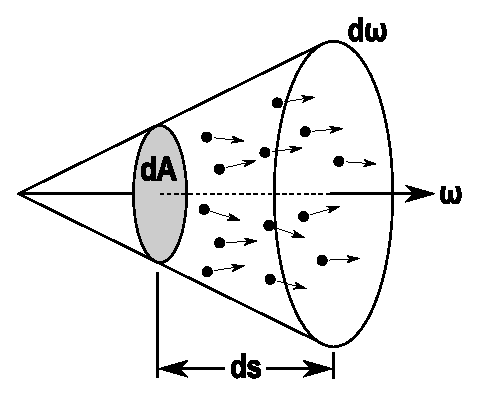
\includegraphics[height=0.3\textheight]{phasespacefluxsurface.eps}
		\caption{Teilchen, die das infinitesimale Flächenelement $dA$ durchqueren und sich in eine Richtung innerhalb des infinitesimalen Raumwinkelelements $d\omega$ um die Flächennormale $\omega$ von $dA$ bewegen.}
		\label{fig:phasespacefluxsurface}
	\end{figure}
	Der Phasenraumfluss ist wie die Phasenraumdichte eine fundamentale Größe, aus der wir alle anderen Observablen ableiten können. Im Folgenden werden wir uns meist auf den Phasenraumfluss beziehen.
		
	Unser Ziel ist es nun eine Bilanzgleichung für Teilchen in einem beliebigen Teil $V \times \Omega$ des Phasenraums (s. Abb.~(\ref{fig:phasespacevolume})) aufzustellen. Dafür sei $V \subset \mathbb{R}^3$ ein Teilvolumen des $\mathbb{R}^3$ und $\Omega \subset \mathcal{S}^2$ ein beliebiger Raumwinkel aus der Einheitskugel $\mathcal{S}^2$. Dazu untersuchen wir Ursachen für eine Veränderung der Teilchenzahl in unserem betrachteten Phasenraumvolumen $V \times \Omega$.
	\begin{figure}
		\centering
		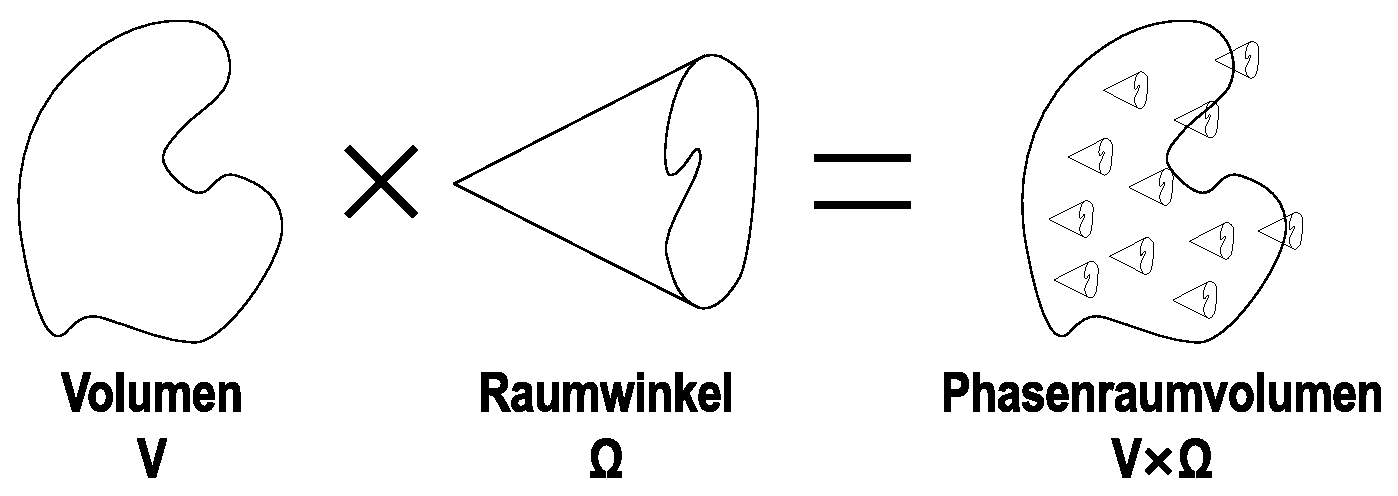
\includegraphics[width=0.8\textwidth]{phasespacevolume.eps}
		\caption{Darstellung einer Teilmenge $V \times \Omega$ des Phasenraums. Sie repräsentiert alle Teilchen, die sich innerhalb des Volumens $V$ befinden und sich in eine Richtung $\omega\in\Omega$ bewegen.}
		\label{fig:phasespacevolume}
	\end{figure}

	Zur {\em Emission} zählt jeder Prozess, der neue Teilchen erzeugt, wie z.B. chemische Reaktionen, thermische Emission oder Kernfusion. Emission innerhalb von $V$ in eine Richtung $\omega\in\Omega$ stellt also eine Quelle für Teilchen dar. Nach der Emission bewegen sich die Teilchen in unserem Modell gradlinig mit konstanter Geschwindigkeit bis eine Wechselwirkung mit dem Medium stattfindet. Bewegt sich ein Teilchen bei seiner gradlinigen Bewegung in das Volumen $V$ hinein oder aus ihm heraus und bewegt es sich dabei in eine Richtung innerhalb von $\Omega$, so ändert dies ebenfalls die Bilanz. In diesem Fall sprechen wir von {\em Durchströmen}. Findet eine {\em Kollision} des Teilchens mit dem Medium statt, kann das Teilchen entweder absorbiert oder gestreut werden. Wird es absorbiert wirkt dies als Teilchensenke. Wird es gestreut, dann kann es, je nach Richtung vor und nach der Kollision, entweder keinen Einfluss auf die Teilchenbilanz haben (Bewegungsrichtung vor und nach der Kollision entweder innerhalb oder außerhalb von $\Omega$), es kann herausgestreut werden (Bewegungsrichtung vor der Kollision innerhalb und nach der Kollision ausserhalb von $\Omega$) oder aber hineingestreut werden (Bewegungsrichtung vor der Kollision ausserhalb und nach der Kollision innerhalb von $\Omega$) werden.
	
	Um die einzelnen Beiträge dieser Prozesse zur Teilchenbilanz quantitativ zu erfassen führen wir die Teilchenzahl $$N(t):=\int_\Omega \int_V n(\location{r},\omega,t)\,d\location{r}\,d\omega$$ ein. Sie gibt an wieviele Teilchen sich zum Zeitpunkt $t$ im Phasenraumvolumen $V \times \Omega$ befinden. Durch die eben beschriebenen Prozesse ändert sich $N(t)$ normalerweise mit der Zeit. Ist die Zeit, die ein Teilchen benötigt um das System zu durchqueren, klein gegenüber der typischen Zeitskala für Veränderung des Systems, können wir annehmen, dass sich die Teilchenzahl überall im dynamischen Gleichgewicht befindet, d.h. dass Teilchen ständig aus dem Phasenraumvolumen hinein- und hinausströmen, erzeugt, absorbiert und gestreut werden, aber sich alle Prozesse die Waage halten, $N(t)$ also stationär ist:$$\frac{dN}{dt}=0\qquad\left[\frac{1}{\text{s}}\right].$$ Teilen wir diese Änderung von $N$ mit der Zeit auf die erläuterten Prozesse auf, sind wir bei der Bilanzgleichung angelangt:$$\frac{dN}{dt}=\begin{bmatrix}\text{Änderung}\\ \text{durch}\\ \text{Emission}\end{bmatrix}+\begin{bmatrix}\text{Änderung}\\ \text{durch}\\ \text{Durchströmung}\end{bmatrix}+\begin{bmatrix}\text{Änderung}\\ \text{durch}\\ \text{Kollisionen}\end{bmatrix}=0.$$ Wir leiten nun für jeden dieser Ausdrücke einen Formelausdruck her.
	Die Änderung aufgrund von Emission nennen wir $$\mathbf{E}=\int_\Omega \int_V q(\location{r},\omega)\,d\location{r}\,d\omega\qquad\left[\frac{1}{\text{s}}\right],$$ wobei wir die Quellfunktion $q$ (mit Einheit $\text{m}^{-3}\text{sr}^{-1}\text{s}^{-1}$) eingeführt haben, die für jeden Ort $\location{r}$ und jede Raumrichtung $\omega$ die Anzahl pro Sekunde, Einheitsvolumen und Einheitsraumwinkel erzeugter Teilchen angibt. Hinein- und herausströmende Teilchen erzeugen eine Teilchenrate
	$$\mathbf{S}=\int_\Omega \int_{\partial V} \phi(\location{r},\omega)(\omega \cdot \location{n}(\location{r}))d\location{r}\,d\omega,$$
	die wir durch Integrieren über $\partial V$ (die Oberfläche von V) erhalten. Hierbei steht $\location{n}(\location{r})$ für die Flächennormale am Ort $\location{r}\in\partial V$. Das Skalarprodukt zwischen Bewegungsrichtung $\omega$ und Flächennormalen sorgt für das richtige Vorzeichen, wobei ein positiver Wert Teilchenverlust bedeutet.
	Der letzte Beitrag $\mathbf{C}$ trägt den Kollisionen Rechnung. Da Teilchen nur mit dem Medium, nicht aber untereinander interagieren, muss die Kollisionsrate unabhängig von $\phi$ sein. Wir unterteilen $\mathbf{C}$ in einen Absorptionsteil und einen Streuanteil:
	$$\mathbf{C}=\mathbf{C}_\text{abs}+\mathbf{C}_\text{sca}.$$
	Wir nehmen an, dass die Wahrscheinlichkeit einer Absorption proportional zur zurückgelegten Distanz im Medium ist und unabhängig von der Bewegungsrichtung, was gleichbedeutend mit der Annahme eines isotropen Mediums ist. Die Proportionalitätskonstante am Ort $\location{r}$ nennen wir den (Volumen-)Absorptionsquerschnitt $\kappa(\location{r})$ ($[\kappa]=\frac{1}{\text{m}}=\frac{m^2}{m^3}$). Die zugehörige Teilchenrate ist
	$$\mathbf{C}_\text{abs}=\int_\Omega \int_V \kappa(\location{r})\phi(\location{r},\omega)\,d\location{r}\,d\omega.$$
	Die genauen Mechanismen der Streuung werden bei der Lösung der Wellengleichung behandelt (Mie--Theorie). In unserem Teilchentransport repräsentieren wir diese Streumodelle durch die Streuphasenfunktion $k(\location{r},\omega,\omega')$ und den Volumenstreuquerschnitt $\sigma(\location{r})$. Dabei gibt $k(\location{r},\omega,\omega')$ bei Streuung eines aus Richtung $\omega$ kommenden Teilchens am Ort $\location{r}$ die Wahrscheinlichkeit pro Einheitsraumwinkel an, nach $\omega'$ gestreut zu werden. Da ein gestreutes Teilchen erhalten bleibt, gilt für $k$ die Normierungsbedingung
	\begin{equation}\label{eq:k_norm_req}
	  \int_{\mathcal{S}^2} k(\location{r},\omega,\omega')\,d\omega'=1.
	\end{equation}
	Außerdem ist $k$ symmetrisch bezüglich Vertauschung der Bewegungsrichtungen vor und nach der Streuung:
	$$k(\location{r},\omega,\omega')=k(\location{r},\omega',\omega)\quad \forall\:\omega,\omega'\in\mathcal{S}^2.$$
	Beide Bedingungen werden z.B. durch die isotrope Streuphasenfunktion $$k_\text{iso}(\location{r},\omega,\omega')=\frac{1}{4\pi}$$ erfüllt.
	Wie bei der Absorption, nehmen wir an, dass die Wahrscheinlichkeit eines Teilchens gestreut zu werden von der durch das Medium zurückgelegten Distanz, nicht aber von der Bewegungsrichtung abhängt. Wir teilen $\mathbf{C}_\text{sca}$ weiter auf, in einen Teil
	$$\mathbf{C}_\text{out}=\int_\Omega \int_V \int_{\mathcal{S}^2} \sigma{(\location{r})}k(\location{r},\omega,\omega')\phi(\location{r},\omega)\,d\omega'\,d\location{r}\,d\omega,$$
	der herausgestreute Teilchen berücksichtigt, sowie einen Teil
	$$\mathbf{C}_\text{in}=\int_\Omega \int_V \int_{\mathcal{S}^2} \sigma{(\location{r})}k(\location{r},\omega',\omega)\phi(\location{r},\omega')\,d\omega'\,d\location{r}\,d\omega$$
	entsprechend für hineingestreute Teilchen. Dabei sollte erwähnt werden, dass sowohl $\mathbf{C}_\text{out}$ als auch $\mathbf{C}_\text{in}$ Teilchen berücksichtigen, deren Richtung vor und nach der Streuung in $\Omega$ liegt, was weder einem Zuwachs noch einem Verlust an Teilchen entspricht. Da für unsere Bilanz aber immer nur die Differenz von $\mathbf{C}_\text{out}$ und $\mathbf{C}_\text{in}$ betrachtet wird, hebt sich dieser Teil wieder heraus. Alternativ könnten wir auch über $\mathcal{S}^2 \setminus \Omega$ integrieren, was zu einer komplizierteren Rechnung, aber zu keinem anderen Endergebnis führen würde. Fügen wir die Einzelterme zusammen und ordnen nach Zuwächsen und Verlusten sieht unsere Bilanzgleichung für die Teilchenraten in $V \times \Omega$ wie folgt aus:
	$$\underbrace{\mathbf{S}+\mathbf{C}_\text{abs}+\mathbf{C}_\text{out}}_\text{Verluste}=\underbrace{\mathbf{E}+\mathbf{C}_\text{in}}_\text{Zuwächse}$$
	Es fällt bei der Betrachtung der Formeln für die einzelnen Terme auf, dass alle Terme bis auf $\mathbf{S}$ Volumenintegrale über $V$ enthalten. $\mathbf{S}$ enthält stattdessen ein Oberflächenintegral über $\partial V$. Mit dem Gauss'schen Satz erhalten wir
	$$\mathbf{S}=\int_\Omega \int_V \omega \cdot (\nabla\phi)(\location{r},\omega)\,d\location{r}\,d\omega,$$
	wobei wir $$\nabla \cdot(\omega\phi)=\omega\cdot(\nabla\phi)+\underbrace{(\nabla\omega)}_{=0}\cdot\,\phi$$ benutzt haben.
	
	In der Bilanzgleichung treten jetzt nur noch Volumenintegrale über $V \times \Omega$ auf. Da $V$ und $\Omega$ beliebig gewählt waren, erhalten wir den lokalen Zusammenhang:
	\begin{multline*}
	  \omega\cdot\nabla\phi(\location{r},\omega)+\kappa(\location{r})\phi(\location{r},\omega)+\int_{\mathcal{S}^2}\sigma(\location{r})k(\location{r},\omega,\omega')\phi(\location{r},\omega)d\omega' \\
	  =q(\location{r},\omega)+\int_{\mathcal{S}^2}\sigma(\location{r})k(\location{r},\omega',\omega)\phi(\location{r},\omega')d\omega'.
	\end{multline*}
	Da beim $\mathbf{C}_\text{out}$--Integral $\sigma$ und $\phi$ nicht von der Integrationsvariable abhängen und sich das verbleibende Integral aufgrund der Normierung (\ref{eq:k_norm_req}) vereinfacht, ergibt sich schließlich die Bilanzgleichung in Gestalt einer Integro--Differentialgleichung in $\phi$:
	\begin{equation}\label{eq:particle_balance_equation}
	  \omega\cdot\nabla\phi(\location{r},\omega)+\left(\kappa(\location{r})+\sigma(\location{r})\right)\phi(\location{r},\omega)
	  =q(\location{r},\omega)+\sigma(\location{r})\int_{\mathcal{S}^2}k(\location{r},\omega',\omega)\phi(\location{r},\omega')d\omega'
	\end{equation}
	Im folgenden Abschnitt stellen wir den Bezug zwischen unseren abstrakten Teilchentransportgrößen und physikalischen Strahlungsgrößen her.

	\section{Phänomenologische Strahlungsgrößen}\label{subsec:strahlungsgroessen}
	Im vorigen Abschnitt haben wir das Strahlungstransportproblem bewusst auf ein Teilchentransportproblem (mit abstrakten Teilchen statt Photonen) reduziert um einerseits eine klare Herleitung zu ermöglichen und um andererseits die Verwandtschaft zu anderen Transportproblemen (wie z.B. Neutronentransport) offensichtlich zu machen. Für den Anschluss zu radiometrischen Strahlungsgrößen, ersetzen wir die abstrakten Teilchen durch Photonen. Photonen haben zwei Eigenschaften die wir berücksichtigen müssen. Sie bewegen sich konstant mit Lichtgeschwindigkeit, d.h. wir können die vorher gebrauchte allgemeine Teilchengeschwindigkeit $v$ gleich $\text{c}$ setzen. Außerdem besitzt jedes Photon eine Energie, die mit seiner Frequenz $\nu$ über 
	$$E=h\nu \qquad[J]$$
	zusammenhängt. Dabei bezeichnet $h$ das Planck'sche Wirkungsquantum.
	Jeder Frequenz $\nu$ können wir ein monochromatisches Transportproblem zuordnen, dessen Lösung in Form eines Phasenraumflusses $\phi_\nu$ die Photonenfrequenz als Index trägt.
	Die {\em spezifische Intensität} $I_\nu(\location{r},\omega)$ erhalten wir nun aus dem Phasenraumfluss bzw. der Phasenraumdichte gemäß
	\begin{align}\label{eq:intensity_def}
		I_\nu(\location{r},\omega)d\nu & = h\nu\,\phi_\nu(\location{r},\omega)\\
		                       & = c h\nu\,n_\nu(\location{r},\omega) \qquad \left[\frac{\text{W}}{\text{m}^2\text{sr}}\right] \nonumber
	\end{align}
	Sie gibt an, wieviel Joule am Ort $\location{r}$ pro Sekunde durch eine Einheitsfläche mit Flächennormale $\omega$ pro Einheitsraumwinkel in Richtung $\omega$ und pro Frequenzintervall durch Photonen mit Frequenz $\nu$ transportiert wird:
	$$dE_\nu=I_\nu(\location{r},\omega) dA\,dt\,d\omega\,d\nu.$$
	Wir führen außerdem die {\em spezifische Emissivität} $\varepsilon_\nu$ ein. Wir erhalten Sie aus der Quellfunktion $q_\nu$ durch
	\begin{equation}\label{eq:emissivity_def}
		\varepsilon_\nu(\location{r},\omega)d\nu = h\nu\,q_\nu(\location{r},\omega) \qquad \left[\frac{\text{W}}{\text{m}^3\text{sr}}\right].
	\end{equation}
	
	Multiplizieren wir die abstrakte Transportgleichung (\ref{eq:particle_balance_equation}) mit $h\nu$ und benutzen wir die Beziehungen (\ref{eq:intensity_def}, \ref{eq:emissivity_def}) erhalten wir mit
	\begin{equation}\label{eq:stg_diff}
	  \omega\cdot\nabla I_\nu(\location{r},\omega)+\left(\kappa_\nu(\location{r})+\sigma_\nu(\location{r})\right)I_\nu(\location{r},\omega)
	  =\varepsilon_\nu(\location{r},\omega)+\sigma_\nu(\location{r})\int_{\mathcal{S}^2}k_\nu(\location{r},\omega',\omega)I_\nu(\location{r},\omega')d\omega'
	\end{equation}
	die {\em Strahlungstransportgleichung in differentieller Form}. Sie stellt eine Integro--Differentialgleichung für $I_\nu$ auf dem 5--dimensionalen Phasenraum $\mathbb{R}^3 \times \mathcal{S}^2$ dar und kann für jede Frequenz $\nu$ getrennt gelöst werden. Sie gibt für jede Kombination aus Ort $\location{r}$ und Ausbreitungsrichtung $\omega$ das lokal zu erfüllende Gleichgewicht aus Verlusten (linke Seite) und Zuwächsen (rechte Seite) an.
	
	Wir fassen die Verluste durch Absorption und Streuung mit dem {\em Vo\-lu\-men\-ex\-tink\-ti\-ons\-quer\-schnitt}
	$$\xi_\nu(\location{r}):=\kappa_\nu(\location{r})+\sigma_\nu(\location{r}) \qquad\left[\frac{1}{m}\right]$$
	zusammen, wodurch wir (\ref{eq:stg_diff}) auch kürzer als
	\begin{equation}\label{eq:stg_diff2}
	  \omega\cdot\nabla I_\nu(\location{r},\omega)+\xi_\nu(\location{r})I_\nu(\location{r},\omega)
	  =\varepsilon_\nu(\location{r},\omega)+\sigma_\nu(\location{r})\int_{\mathcal{S}^2}k_\nu(\location{r},\omega',\omega)I_\nu(\location{r},\omega')d\omega'
	\end{equation}
	schreiben können.
	Außerdem definieren wir die dimensionslose {\em optische Tiefe}
	\begin{equation*}
		\tau_\nu(\location{r}_1,\location{r}_2):=\int_{s=0}^{\|\location{r}_2-\location{r}_1\|} \xi_\nu(\location{r}_1+s(\location{r}_2 - \location{r}_1))\,ds,
	\end{equation*}
	als Maß für die Undurchsichtigkeit des Mediums bei der Frequenz $\nu$ zwischen zwei Orten $\location{r}_1$ und $\location{r}_2$. Vereinfachen wir Gleichung (\ref{eq:stg_diff2}), indem wir Quellen zu Null setzen und eine beliebige Richtung $\omega$ wählen, so gelangen wir zur gewöhnlichen Differentialgleichung
	$$I_\nu'(s)+\xi_\nu(s)I_\nu(s)=0,$$
	die durch
	\begin{equation}
		I_\nu(s)=I_\nu(0)\:\text{exp}\left(-\int_{s'=0}^s \xi_\nu(s')\right)=I_\nu(0)\:\text{exp}\left(-\tau_\nu(0,s)\right)
		\label{eq:exponentialdecay}
	\end{equation}
	gelöst wird. Die optische Tiefe beschreibt also eine exponentielle Abschwächung einfallender Intensität. Nach der Definition der verschiedenen phänomenologischen Strahlungsgrößen schauen wir uns nun an, wie ihre Messung aufgefasst und mathematisch definiert werden kann.
	
	
	\section{Die Messgleichung}\label{sec:measurement_equation}
	Mit dem Strahlungsintensitätsfeld, das aus der Gesamtheit aller spezifischen Intensitäten $I_\nu$ besteht, meinen wir die Funktion
	$$I:\mathbb{R}_+\times\mathbb{R}^3\times\mathcal{S}^2\to\mathbb{R}_+\;,\qquad (\nu,\location{r},\omega)\mapsto I_\nu(\location{r},\omega),$$
	die vom 6--dimensionalen Raum aller Frequenzen, Orte und Raumrichtungen auf die lokale spezifische Intensität abbildet.
	
	Funktionen dieser Art bilden einen Skalarproduktraum. Das Null--Element ist die konstant auf Null abbildende Funktion. Zwei Funktionen lassen sich punktweise addieren und ergeben so eine neue Funktion, die auch nach $\mathbb{R}_{\geq 0}$ abbildet. Das Skalarprodukt zwischen zwei Funktionen $f$ und $g$ ist schließlich mit
	$$\langle f,g\rangle=\int_{\mathbb{R}_+} \int_{\mathbb{R}^3} \int_{\mathcal{S}^2} f(\nu,\location{r},\omega)g(\nu,\location{r},\omega)\,d\omega\,d\location{r}\,d\nu$$
	gegeben.
	
	Mit diesem funktionalanalytischen Handwerkszeug definieren wir eine Messung als das Skalarprodukt zwischen unserem Strahlungsintensitätsfeld $I$ und einer {\em Sensitivitätsfunktion} $W$, welche die Stärke der Gewichtung angibt, mit der die spezifische Intensität der Frequenz $\nu$ am Ort $\location{r}$ in Richtung $\omega$ in den Messwert eingeht. Die entsprechende Formel
	\begin{equation}\label{eq:messgleichung}
		M^{(i)}:=\langle W^{(i)},I\rangle=\int_{\mathbb{R}_+} \int_{\mathbb{R}^3} \int_{\mathcal{S}^2} W^{(i)}(\nu,\location{r},\omega)I_\nu(\location{r},\omega)\,d\omega\,d\location{r}\,d\nu
	\end{equation}
	nennen wir {\em Messgleichung} (für den $i$--ten Sensor). Für monochromatische Messungen führen wir zusätzlich noch 
	\begin{equation}\label{eq:messgleichung_mono}
		M_\nu^{(i)}:=\langle W_\nu^{(i)},I_\nu\rangle=\int_{\mathbb{R}^3} \int_{\mathcal{S}^2} W_\nu^{(i)}(\location{r},\omega)I_\nu(\location{r},\omega)\,d\omega\,d\location{r}
	\end{equation}
	ein, womit wir (\ref{eq:messgleichung}) auch als
	\begin{equation}\label{eq:messgleichung_frommonos}
		M^{(i)}=\int_{\mathbb{R}_+} M_\nu^{(i)}\,d\nu
	\end{equation}
	schreiben können.
	Diese Abstraktion erlaubt uns größtmögliche Freiheit beim kreieren virtueller Sensoren. Beispielsweise könnte $W$ nur in einem kleinen Volumen und einem kleinen Raumwinkel, aber bei allen Frequenzen, nichtverschwindend sein, und so einen Sensor zur Messung der Gesamt--Intensität an einem bestimmten Ort in eine bestimmte Richtung repräsentieren. Ebenso kann durch gleichstarke Gewichtung aller Raumrichtungen die mittlere Intensität gemessen werden.
	
	Was zunächst nur als theoretisches Konstrukt ohne praktischen Nutzen erscheint, wird sich später in Verbindung mit Monte--Carlo--Sampling als vielseitiges und effizientes Werkzeug erweisen.
	
	
	\section{Übersicht etablierter Lösungsverfahren}
	TODO: Übersicht benutzter Lösungsverfahren, Meilensteine (wann zum ersten mal Polarisation gerechnet?, Warum etablieren sich MC-Verfahren so spät?, etc...)
		
	\chapter{Pfadintegralformulierung der Strahlungstransportgleichung}\label{chapter:path_radiative_transfer}
	In diesem Abschnitt leiten wir eine alternative mathematische Formulierung der Strahlungstransportgleichung einerseits und ihrer Lösung (genau genommen, Messungen der Lösung im Sinne von (\ref{eq:messgleichung})) andererseits her. Dies führt uns durch die verschiedenen auf das Problem eingenommenen Blickwinkel zu einem besseren Verständnis von Strahlungstransport und gibt uns darüber hinaus einen neuen Ansatzpunkt zur effizienten Lösung des Strahlungstransportproblems.
	
	Die Idee zu dieser Formulierung kommt aus der Dissertation von \citet{Veach:1997p9136}, wird aber schon in \citep{Arvo:1995p9257} vorgestellt. Beide Dissertationen behandeln allerdings nur den Strahlungstransport zwischen Oberflächen. In der Arbeit von \citet{Pauly:2000p5705} wird dies auf partizipierende Medien ausgedehnt. Aus \citep{Arvo:1993p9035} stammt außerdem die Herleitung der integralen Form der Strahlungstransportgleichung.
	
	
	\section{Strahlungstransportgleichung in integraler Form}
	In differentieller Form nimmt die Strahlungstransportgleichung, wie wir in Abschnitt (\ref{subsec:strahlungsgroessen}) gesehen haben, folgende Gestalt an:
		\begin{equation}
			\omega \cdot \nabla I(\location{r},\omega)+\overbrace{\left(\kappa(\location{r})+\sigma(\location{r})\right)}^{=:\xi(\location{r})}I(\location{r},\omega)=\varepsilon(\location{r},\omega)+\sigma(\location{r}) \int_{\mathcal{S}^2} k(\location{r},\omega',\omega)I(\location{r},\omega') d\omega'.
			\label{eq:diff.STG}
		\end{equation}
	Für diesen und die folgenden Abschnitte lassen wir dabei den Index $\nu$ aus übersichtsgründen weg, womit gemeint ist, dass wir stellvertretend für alle Frequenzen ein einzelnes monochromatisches Strahlungstransportproblem einer beliebigen Frequenz nehmen. Wenn wir zum polychromatischen Fall zurückkehren führen wir die Indizes wieder ein.
	
	Schreiben wir das Skalarprodukt zwischen $\omega$ und dem $\nabla$--Operator als Richtungsableitung
	\newcommand{\dds}{\frac{\text{d}}{\text{d}s}}
	\newcommand{\ddszero}{\left. \dds \right|_{s=0}}
	\begin{equation*}
		\omega \cdot \nabla I(\location{r},\omega)
		=  \ddszero I(\location{r}+s\,\omega,\omega)
		=  -\ddszero I(\location{r}-s\,\omega,\omega)
	\end{equation*}
	können wir (\ref{eq:diff.STG}) als
	\begin{multline}
		\dds I(\location{r}-s\,\omega,\omega) - \xi(\location{r}-s\,\omega)I(\location{r}-s\,\omega,\omega) = \\-\varepsilon(\location{r}-s\,\omega,\omega) -\sigma(\location{r}-s\,\omega) \int_{\mathcal{S}^2} k(\location{r}-s\,\omega,\omega',\omega)I(\location{r}-s\,\omega,\omega') \text{d}\omega'
		\label{eq:diff.STGtranslated}
	\end{multline}
	umschreiben. Dabei haben wir die Beschränkung $s=0$ fallengelassen, was die Korrektheit der Umformung aber nicht ändert. Mit den Abkürzungen
	\begin{align*}
		{\hat I}(s)&:=I(\location{r}-s\,\omega,\omega) \\
		Q(\location{r},\omega)&:= \varepsilon(\location{r},\omega)+\sigma(\location{r}) \int_{\mathcal{S}^2} k(\location{r},\omega',\omega)I(\location{r},\omega') d\omega' \\
		{\hat Q}(s)&:=Q(\location{r}-s\,\omega,\omega)\\
		{\hat \xi}(s)&:=\xi(\location{r}-s\,\omega) \\
		{\hat \tau}(s)&:= \int_{s'=0}^{s} {\hat \xi}(s') \text{d}s'
	\end{align*}
	wird aus (\ref{eq:diff.STGtranslated})
	\begin{equation}
		\dds {\hat I}(s) - {\hat \xi}(s){\hat I}(s)= -{\hat Q}(s) \qquad |\cdot e^{-{\hat \tau}(s)}.
		\label{eq:diff.STGhatted}
	\end{equation}
	Gleichung (\ref{eq:diff.STGhatted}) ist eine gewöhnliche Differentialgleichung die sich mit
	\begin{align}
		(\ref{eq:diff.STGhatted})\Leftrightarrow\qquad \dds \left(e^{-{\hat \tau}(s)} {\hat I}(s)\right)&= -e^{-{\hat \tau}(s)} {\hat Q}(s) \qquad | \int_{s'=0}^s (\cdot)\text{d}s' \nonumber \\
		\Leftrightarrow\qquad e^{-{\hat \tau}(s)} {\hat I}(s) - {\hat I}(0) &= -\int_{s'=0}^s e^{-{\hat \tau}(s')} {\hat Q}(s') \text{d}s' \nonumber \\
		\Leftrightarrow\qquad {\hat I}(0) &= e^{-{\hat \tau}(s)} {\hat I}(s) + \int_{s'=0}^s e^{-{\hat \tau}(s')} {\hat Q}(s') \text{d}s' \label{eq:diff.STGpreintegral}
	\end{align}
	leicht nach ${\hat I}(0)$ auflösen lässt. Obwohl ${\hat Q}(s)$ lokal die Intensität $I$ über alle Raumrichtungen integriert, dürfen wir für die Lösung von (\ref{eq:diff.STGhatted}) $Q$ als unabhängig von $I$ behandeln, da die Schnittmenge zwischen der Geraden im Raum, auf der wir die Differentialgleichung lösen, und der Menge aller Raumrichtungen $\mathcal{S}^2$ bei der Integration über alle Raumrichtungen eine Nullmenge ist und somit für physikalisch relevante Strahlungsintensitätsfelder (d.h. solche, die hinreichend stetig/beschränkt bzw. keine Delta--Distribution sind) keinen Beitrag zum Integral leistet.
	Setzen wir in (\ref{eq:diff.STGpreintegral}) für die Abkürzungen wieder die ursprünglichen Ausdrücke ein, erhalten wir die {\em Strahlungstransportgleichung in integraler Form}:
	\begin{multline}
		I(\location{r},\omega) = e^{-\tau(\location{r},\location{r}-s\,\omega)} {\hat I}(\location{r},\location{r}-s\,\omega) + \int_{s'=0}^\infty e^{-\tau(\location{r},\location{r}-s\,\omega)} \;\cdot \\
		\quad\cdot\left( \varepsilon(\location{r}-s'\,\omega,\omega) + \sigma(\location{r}-s'\,\omega)
		\left[ \int_{\mathcal{S}^2} k(\location{r}-s'\,\omega,\omega',\omega)I(\location{r}-s'\,\omega,\omega') \text{d}\omega'\right] \right) \text{d}s'
		\label{eq:int.STG}
	\end{multline}
	Nehmen wir nun als Randbedingungen an, dass in unendlich großer Entfernung keine Lichtquellen existieren, d.h. $\forall \omega \in \mathcal{S}^2 : I(\location{r}=-\infty\cdot\omega,\omega)=0$, dann vereinfacht sich (\ref{eq:int.STG}) zu
	\begin{multline}
		I(\location{r},\omega) = \int_{s'=0}^\infty e^{-\tau(\location{r},\location{r}-s\,\omega)} \;\cdot \\
		\quad\cdot\left( \varepsilon(\location{r}-s'\,\omega,\omega) + \sigma(\location{r}-s'\,\omega)
		\left[ \int_{\mathcal{S}^2} k(\location{r}-s'\,\omega,\omega',\omega)I(\location{r}-s'\,\omega,\omega') \text{d}\omega'\right] \right) \text{d}s'
		\label{eq:int.STGdarkbg}
	\end{multline}


	\section{Strahlungstransportgleichung in Operator--Form}
	Schauen wir uns die einzelnen Teile der Gleichung (\ref{eq:int.STGdarkbg}) genauer an.
	Der innere Teil von (\ref{eq:int.STGdarkbg}) in eckigen Klammern summiert an einem festen Ort ($\location{r}-s'\,\omega$), mit der Streuphasenfunktion $k$ gewichtet, die einfallenden Intensitäten auf, die in Richtung $\omega$ gestreut werden. Anschließend skaliert der Volumenstreuquerschnitt die aufintegrierte Intensität entsprechend dem lokal vorhandenen Medium und gibt dabei dem Ausdruck die Einheit einer Emissivität.
	Der restliche äußere Teil der Gleichung addiert die eben gewonnene Emissivität durch Einstreuung zu der lokal durch Ausstrahlung erzeugten Emissivität an jedem Punkt auf einer Geraden hinter dem Punkt $\location{r}$ und summiert die mit einem der optischen Tiefe entsprechenden Abschwächungsfaktor gewichteten, in Richtung $\omega$ zeigenden, Emissivitäten, entlang der Geraden zur Gesamtintensität am Ort $\location{r}$ in Richtung $\omega$ auf.
	Der Gesamtausdruck lässt sich durch Einführung zweier neuer Operatoren
	\begin{align*}
		\left(\mathbf{G}\varepsilon\right)(\location{r},\omega)&:=\int_{s'=0}^\infty e^{-\tau(\location{r}-s' \omega,\location{r})}\varepsilon(\location{r}-s' \omega,\omega) ds' \\
		\left(\mathbf{K}I\right)(\location{r},\omega)&:=\sigma(\location{r})\int_{S^2} k(\location{r},\omega',\omega) I(\location{r},\omega') d\omega'
	\end{align*}
	\begin{equation*}
		\mathbf{G} : \varepsilon(\location{r},\omega) \mapsto I(\location{r},\omega) , \qquad
		\mathbf{K} : I(\location{r},\omega) \mapsto \varepsilon(\location{r},\omega)
	\end{equation*}
	in elementarere Prozesse aufteilen. Wir nennen $\mathbf{G}$ den sogenannten {\em Fortpflanzungs--Operator} und $\mathbf{K}$ den {\em Streu--Operator}. Beides sind Integraloperatoren auf dem Raum der Funktionen $f : \mathbb{R}^3 \times \mathcal{S}^2 \to \mathbb{R}_+$, die vom Teilchen--Phasenraum auf die positiven reellen Zahlen abbilden. Beide haben komplementäre Lokalitäten. Während $\mathbf{K}$ lokal im Ort über alle Raumrichtungen integriert, ist $\mathbf{G}$ lokal in der Raumrichtung und integriert über alle Orte entlang einer Geraden im Raum. Dabei bildet $\mathbf{K}$ von einem Strahlungsintensitätsfeld auf ein Emissivitätsfeld ab. Bei $\mathbf{G}$ ist es umgekehrt, es macht aus einem Emissivitätsfeld wieder ein Strahlungsintensitätsfeld.
	Mit diesen neuen Operatoren wird aus Gleichung (\ref{eq:int.STGdarkbg}) die {\em Operatorform der Strahlungstransportgleichung}
	\begin{equation}
		I=\mathbf{G}(\varepsilon + \mathbf{K}I),
		\label{eq:op.STG}
	\end{equation}
	die wir nach $I$ auflösen können:
	\begin{align}
		(\ref{eq:op.STG}) \Leftrightarrow I&=\mathbf{G}\varepsilon + \mathbf{GK}I \nonumber \\
		\Leftrightarrow (\mathbf{1}-\mathbf{GK})I &= \mathbf{G}\varepsilon \nonumber \\
		\Leftrightarrow I &= (\mathbf{1}-\mathbf{GK})^{-1}\mathbf{G}\varepsilon \label{eq:op.STGinvert} \\
		\Leftrightarrow I &= \sum_{k=0}^\infty (\mathbf{GK})^k \mathbf{G}\varepsilon \label{eq:op.STGneumann} \\
		&=\mathbf{G}\varepsilon + \mathbf{GKG}\varepsilon + \mathbf{GKGKG}\varepsilon + \hdots \label{eq:op.STGneumann.explicit} \\
		\Leftrightarrow I &=\sum_{k=0}^\infty \mathbf{G} (\mathbf{KG})^k \varepsilon \label{eq:op.STGkg}
	\end{align}
	Damit ist das Strahlungstransportproblem formal gelöst! Dabei haben wir den auftretenden invertierten Operator (\ref{eq:op.STGinvert}) durch eine Neumann--Reihe (\ref{eq:op.STGneumann}) ersetzt. Dies ist dann zulässig wenn die Operatornorm des Operators $\mathbf{GK}$ kleiner als eins ist und damit sichergestellt ist, dass die Neumann--Reihe konvergiert. Für alle praktisch relevanten Probleme ist dies der Fall \citep[s.][Theorem 12 und 13]{Arvo:1995p9257}. Physikalisch lässt sich das Gleichgewichts--Strahlungsintensitätsfeld als Summe aus Intensitätsfeldern verstehen, die durch Photonen mit unterschiedlich vielen Streuereignissen auf ihrem Weg von der Emission aus einer Lichtquelle bis zu ihrer Messung mit einem Messinstrument entstanden sind (wie in Schritt (\ref{eq:op.STGneumann.explicit}) deutlich wird). Dabei müssen Pfade jeder möglichen Länge (sprich Anzahl an Streuereignissen) berücksichtigt werden. Zwischen Emission und Messung wechseln sich dabei Fortpflanzung $\mathbf{G}$ und Streuung $\mathbf{K}$ ab. Im letzen Schritt (\ref{eq:op.STGkg}) haben wir $\mathbf{G}$ nach links ausgeklammert um den $\mathbf{KG}$--Operator herauszustellen.
	
	
	\section{KG--Operator in Volumenform}
	Schauen wir uns den $\mathbf{KG}$--Operator genauer an. Nachdem $\mathbf{KG}$ ein Emissivitätsfeld durch Fortpflanzung zu einem Intensitätsfeld aufintegriert hat, wird dieses durch die anschliessende Streuung erneut auf ein Emissivitätsfeld abgebildet:
	\begin{equation*}
		\mathbf{KG} : \varepsilon(\location{r},\omega) \mapsto \varepsilon(\location{r},\omega)
	\end{equation*}

	Setzen wir die Definitionen der Operatoren ein und fassen die Integrale zusammen:
	\begin{align*}
		\left(\mathbf{KG}\varepsilon\right)(\location{r},\omega)&=\sigma(\location{r}) \int_{\mathcal{S}^2} k(\location{r},\omega',\omega)\left[\int_{s'=0}^\infty e^{-\tau(\location{r}-s' \omega',\location{r})}\varepsilon(\location{r}-s' \omega',\omega') \text{d}s'\right] \text{d}\omega' \\
		&=\sigma(\location{r}) \int_{\mathcal{S}^2} \int_{s'=0}^\infty k(\location{r},\omega',\omega) e^{-\tau(\location{r}-s' \omega',\location{r})}\varepsilon(\location{r}-s' \omega',\omega') \underbrace{\text{d}s' \text{d}\omega'}_{=\frac{\text{d}\location{r}'}{s'^2}} \\
		&=\sigma(\location{r}) \int_{\mathbb{R}^3} k(\location{r},\omega',\omega) \frac{e^{-\tau(\location{r}',\location{r})}}{\|\location{r}-\location{r}'\|^2}\varepsilon(\location{r}',\omega') \,\text{d}\location{r}'
	\end{align*}
	Da wir durch Kombination der Integration über alle Raumrichtungen $\omega'$ und alle Entfernungen $s'$ den gesamten Raum abdecken, können wir die beiden Integrale zugunsten eines Volumenintegrals über den gesamten Raum und einen geometrischen Verdünnungsfaktor tauschen. Mit dem Ziel, später alle Integrationen zu Volumenintegralen zusammenzufassen, schreiben wir den $\mathbf{KG}$--Operator so um, dass alle expliziten Angaben von Entfernungen und Raumrichtungen durch eine raumpunktorientierte Notation ersetzt werden:
	\begin{multline}
		\left(\mathbf{KG}\varepsilon\right)(\location{r}_i \rightarrow\location{r}_{i+1})=\\
		\sigma(\location{r}_i) \int_{\mathbb{R}^3} k(\location{r}_{i-1}\rightarrow\location{r}_i\rightarrow\location{r}_{i+1})\frac{e^{-\tau(\location{r}_{i-1},\location{r}_i)}}{\|\location{r}_i-\location{r}_{i-1}\|^2}\varepsilon(\location{r}_{i-1} \rightarrow\location{r}_i)d\location{r}_{i-1}
		\label{eq:KGvolume_intermediate}
	\end{multline}
	Wir führen zusätzlich noch die Abkürzung
	\begin{align*}
		\scatter{i}\;&:=\sigma(\location{r}_i)k(\location{r}_{i-1}\rightarrow\location{r}_i\rightarrow\location{r}_{i+1})\\
			&=\sigma(\location{r}_i)k(\location{r}_i,\normalized{\location{r}_i-\location{r}_{i-1}},\normalized{\location{r}_{i+1}-\location{r}_i})
	\end{align*}
	ein, so dass wir (\ref{eq:KGvolume_intermediate}) zusammen mit den in Abschnitt \ref{subsec:nomenklatur} eingeführten Schreibweisen noch kompakter als
	\begin{equation}
		\left(\mathbf{KG}\varepsilon\right)_{(i,i+1)}=\int_{\mathbb{R}^3} \scatter{i}\frac{e^{-\tau_{(i-1,i)}}}{d_{(i-1,i)}^2}\varepsilon_{(i-1,i)}d\location{r}_{i-1}.
		\label{eq:KGvolume}
	\end{equation}
	schreiben können.


	\section{Pfadintegrallösung der Strahlungstransportgleichung}
	Wir setzen die Neumann--Reihen--Lösung (\ref{eq:op.STGkg}) in die monochromatische Meßgleichung (\ref{eq:messgleichung_mono}) ein und erhalten
	\begin{align}
		M_\nu&=\int_{\mathbb{R}^3}\int_{\mathcal{S}^2}W_\nu(\location{r},\omega) \left(\sum_{k=0}^\infty \mathbf{G} (\mathbf{KG})^k \varepsilon_\nu\right)(\location{r},\omega) \,\text{d}\omega \,\text{d}\location{r} \nonumber \\
		&=\sum_{k=0}^\infty \int_{\mathbb{R}^3}\int_{\mathcal{S}^2}W_\nu(\location{r},\omega) \left(\mathbf{G} (\mathbf{KG})^k \varepsilon_\nu\right)(\location{r},\omega) \,\text{d}\omega \,\text{d}\location{r} \nonumber \\
		&=\sum_{k=0}^\infty \int_{\mathbb{R}^3}\int_{\mathcal{S}^2}W_\nu(\location{r},\omega) \int_{s'=0}^\infty e^{-\tau_\nu(\location{r}-s' \omega,\location{r})} \left((\mathbf{KG})^k \varepsilon_\nu\right)(\location{r},\omega) \underbrace{\text{d}s' \,\text{d}\omega}_{=\frac{\text{d}\location{r}'}{s'^2}} \,\text{d}\location{r} \nonumber \\
		&=\sum_{k=0}^\infty \int_{\mathbb{R}^3}\int_{\mathbb{R}^3}W_\nu(\location{r}'\rightarrow\location{r}) \frac{e^{-\tau_\nu(\location{r}',\location{r})}}{\|\location{r}'-\location{r}\|^2} \left((\mathbf{KG})^k \varepsilon_\nu\right)(\location{r}'\rightarrow\location{r}) \,\text{d}\location{r}' \,\text{d}\location{r}.
		\label{eq:STGprepathsolution}
	\end{align}
	Durch rekursives Einsetzen von (\ref{eq:KGvolume}) in (\ref{eq:STGprepathsolution}) und Neuanordnung der Terme erhalten wir dann als Ergebnis einer monochromatischen Messung:
	\begin{equation}
		M_\nu=\sum_{k=0}^\infty \underbrace{\idotsint}_{(k+2)\text{--mal}}\varepsilon_{\nu,(0,1)}\left[\prod_{i=1}^k\frac{e^{-\tau_{\nu,(i-1,i)}}}{d_{(i-1,i)}^2}\scatter{i}\right]\frac{e^{-\tau_{\nu,(k,k+1)}}}{d_{(k,k+1)}^2} W_{\nu,(k,k+1)} \;\text{d}\location{r}_0 \dotsm \text{d}\location{r}_{k+1} .
		\label{eq:STGpathsolution}
	\end{equation}
	Das Ergebnis ist eine Summe aus reinen $(k+2)$--fachen Volumenintegralen über den ganzen Raum, wobei über den möglichen Start- und Endpunkt sowie die $k$ Streupunkte innerhalb des Photonenpfades integriert wird.
	Anschaulich müssen wir also die Beiträge von Pfaden jeder Anzahl an Streupunkten und jeder möglichen Anordnung von Emissions-, Streu- und Mess\-orten aufsummieren. Dies wird vielleicht klarer, wenn wir die ersten Terme der Summe explizit ausformulieren:
	\begin{align*}
		M_\nu&=\iint_{(\mathbb{R}^3)^2}\varepsilon_{\nu,(0,1)}\frac{e^{-\tau_{\nu,(0,1)}}}{d_{(0,1)}^2} W_{\nu,(0,1)} \;\text{d}\location{r}_0\text{d}\location{r}_1 \\
		&+\iiint_{(\mathbb{R}^3)^3}\varepsilon_{\nu,(0,1)}\frac{e^{-\tau_{\nu,(0,1)}}}{d_{(0,1)}^2}\scatter{1}\frac{e^{-\tau_{\nu,(1,2)}}}{d_{(1,2)}^2} W_{\nu,(1,2)} \;\text{d}\location{r}_0\text{d}\location{r}_1\text{d}\location{r}_2 \\
		&+\iiiint_{(\mathbb{R}^3)^4}\varepsilon_{\nu,(0,1)}\frac{e^{-\tau_{\nu,(0,1)}}}{d_{(0,1)}^2}\scatter{1}\frac{e^{-\tau_{\nu,(1,2)}}}{d_{(1,2)}^2}\scatter{2}\frac{e^{-\tau_{\nu,(2,3)}}}{d_{(2,3)}^2} W_{\nu,(2,3)} \;\text{d}\location{r}_0\text{d}\location{r}_1\text{d}\location{r}_2\text{d}\location{r}_3 \\
		&+\hdots
	\end{align*}
	Diese Form der Lösung des Strahlungstransportproblems hat mehrere Vorteile:
	\begin{itemize}
		\item{Die Lösung besitzt eine anschauliche Interpretation}
		\item{Die Lösung ist explizit, es muss keine implizite Integro--Differentialgleichung wie (\ref{eq:stg_diff}) gelöst werden}
		\item{Die Lösung ist ein reines Integrationsproblem und somit ein gutes Gegenstück zu hochdimensionalen Monte--Carlo--Integrations--Verfahren, wie wir in Abschnitt \ref{subsec:integrationsproblem_comparison} sehen werden}
	\end{itemize}
	Das polychromatische Messergebnis ergibt sich nun einfach durch Einsetzen von (\ref{eq:STGpathsolution}) in (\ref{eq:messgleichung_frommonos}).


	\section{Elimination der Neumann--Reihe}\label{sec:neumann_elimination}
	Unsere Darstellung der Lösung (\ref{eq:STGpathsolution}) des Strahlungstransportproblems besteht bisher aus einer unendlichen Summe von Integralen, was eine direkte Folge der Aufspaltung des Lösungsoperators aus (\ref{eq:op.STGinvert}) in seine Neumann--Reihe (\ref{eq:op.STGneumann}) ist. In dieser Form sind die Pfade in Klassen gleicher Länge (d.h. Anzahl an Streupunkten) eingeteilt, was die mathematische Behandlung vereinfacht, da die Fälle verschiedener Länge getrennt voneinander behandelt werden können. Gleichzeitig verleitet diese Darstellung jedoch dazu zu glauben, es wäre sinnvoll oder läge in der Natur der Sache, die Pfade unterschiedlicher Länge getrennt voneinander zu behandeln. Tatsächlich gibt es aber keinen physikalischen Grund dafür, vielmehr wäre es auch mathematisch hilfreich die Lösung als ein einziges Integral über den Raum aller Pfade darzustellen, da wir es dann formal mit nur noch einem Integrationsproblem zu tun hätten und nicht mehr mit unendlich vielen.
	
	Daher führen wir nun \citet[][8.2]{Veach:1997p9136} folgend, die Menge aller Pfade sowie ein passendes Integrationsmaß ein, um unsere Lösung (\ref{eq:STGpathsolution}) als Einzelintegral darstellen zu können. Sei dazu $\Omega_{\nu,k}$ die Menge aller Pfade der Frequenz $\nu$ und der Länge $k$, d.h. Pfade der Form
	$${\overline x}=\location{r}_0\location{r}_1\cdots\location{r}_k\location{r}_{k+1},$$
	mit $k\in\{0,1,2,\dots\}$ und $\location{r}_i \in \mathbb{R}^3$ für alle $i$. Wir definieren mittels
	$$\mu_k(D)=\int_D d\nu d\location{r}_0\cdots d\location{r}_{k+1}$$
	ein Maß für Pfade der Länge $k$, wobei $D\subset\Omega_k$ eine Teilmenge von Pfaden dieser Länge repräsentiert und $d\location{r}_i$ das geometrische Volumenmaß sowie $d\nu$ das Integrationsmaß über die positiven reellen Zahlen darstellt. Die Menge aller Pfade ist die Vereinigung
	$$\Omega=\bigcup_{k=0}^\infty \Omega_k$$
	der Mengen von Pfaden verschiedener Längen. Daß Maß für die Integration von beliebigen Teilmengen des Pfadraumes $D\subset\Omega$ ist nun durch
	$$\mu(D)=\sum_{k=0}^\infty \mu_k(D\cap\Omega_k)$$
	gegeben, d.h. das Maß für $D$ ist einfach die Summe der Maße von Pfaden aus $D$ entsprechender Länge. Benennen wir nun noch den pfadlängen- und frequenzabhängigen Integranden aus (\ref{eq:STGpathsolution})
	\begin{equation}
		f({\overline x}_\nu)=f_\nu(\location{r}_0\location{r}_1\cdots\location{r}_k\location{r}_{k+1})=\varepsilon_{\nu,(0,1)}\left[\prod_{i=1}^k\frac{e^{-\tau_{\nu,(i-1,i)}}}{d_{(i-1,i)}^2}\scatter{i}\right]\frac{e^{-\tau_{\nu,(k,k+1)}}}{d_{(k,k+1)}^2} W_{\nu,(k,k+1)}
		\label{eq:mcf}
	\end{equation}
	als {\em Messbeitragsfunktion} $f$, dann können wir nun die polychromatische Messung (\ref{eq:messgleichung}) einfach als
	\begin{equation}
		M=\int_\Omega f({\overline x})d\mu({\overline x})
		\label{eq:unified_measurementintegral}
	\end{equation}
	schreiben. Es ist in dieser Form leichter einzusehen, dass wir die Pfade nicht nach ihrer Länge zusammengefasst behandeln müssen, um anschließend die (unendlich vielen) Ergebnisse aufzusummieren, sondern stattdessen Pfade in beliebiger Weise zur Integration zusammenfassen dürfen. Dies ist insbesondere für die Monte--Carlo--Integration wichtig, da unsere ganze Theorie sich dort auf die Lösung eines Einzelintegrals beschränken wird und wir dadurch dort nahtlos mit der Lösung von Messintegralen der Form (\ref{eq:unified_measurementintegral}) anknüpfen können.

		\section{Monte--Carlo--Integration}
	Monte--Carlo--Verfahren liegt die Idee zugrunde, zu einem numerischen Problem ein passendes Zufallsexperiment so zu konstruieren, da"s der Erwartungswert einer Zufallsvariable des Experiments das numerische Problem l"ost.
	
	Die Idee ist nicht neu, so f"uhrte {\em Buffon} 1777 folgendes Experiment durch: Eine Nadel der L"ange $L$ wird wiederholt auf eine plane Fl"ache mit parallelen Linien im Abstand $d>L$ fallengelassen und jeweils notiert, ob die Nadel eine der Linien kreuzt. Er zeigte, da"s der Erwartungswert f"ur die Wahrscheinlichkeit der Nadel, die Linie zu kreuzen $$p=\frac{2L}{\pi d}$$ betr"agt. Laplace wies sp"ater darauf hin, da"s  man die H"aufigkeit, mit der die Nadeln die Linien kreuzen, auch Nutzen kann, um den Wert von $\pi$ zu sch"atzen (siehe Abb. \ref{fig:buffon}): $$\pi=\frac{2L}{p d}\approx \frac{2L}{\frac{k}{N}d}$$
	(\text{N Experimente, davon k mal eine Linie gekreuzt}).
	\begin{figure}
		\centering
		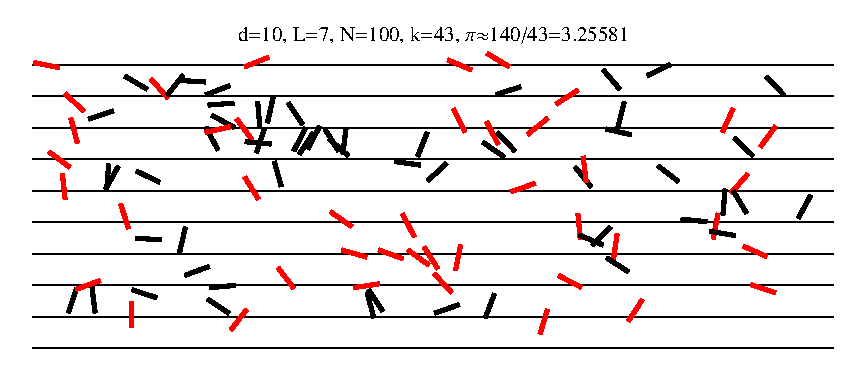
\includegraphics[height=0.3\textheight]{buffonsneedles.eps}
		\caption{Beispiel f"ur eine Realisierung des Buffon--Nadel--Experiments mit 100 geworfenen Nadeln. Der erhaltene Sch"atzwert f"ur $\pi$ ist bei so wenigen Nadeln nicht sehr genau.}
		\label{fig:buffon}
	\end{figure}
	
	\subsection{Das Integrationsproblem}\label{subsec:integrationsproblem}
	Betrachten wir das Integral
	\begin{equation}
		I=\int_\Omega f(x) d\mu(x),
		\label{eq:integration_problem}
	\end{equation}
	wobei $\Omega$ das Integrationsgebiet, $f : \Omega \to \mathbb{R}$ eine reellwertige Funktion und $\mu$ ein Ma"s auf $\Omega$ ist. F"ur die folgende Darstellung nehmen wir an, da"s $$\Omega=[0,1]^d$$ der $d$--dimensionale Einheitsw"urfel und $I_d$ das zugeh"orige Integral ist.
	\subsubsection{Klassische numerische Quadraturverfahren}
	Die klassische numerische Herangehensweise (wenn keine analytische L"osung m"oglich oder praktikabel ist) sind {\em Tensor--Produkt--Verfahren}. Die Idee dabei ist, f"ur jede Dimension ein eindimensionales Quadratur--Verfahren zu w"ahlen (verschiedene oder das gleiche) und diese zu einem mehrdimensionalen Verfahren zu kombinieren. Ein eindimensionales Verfahren stellt eine gewichtete Summe von Funktionswerten an $M$ (vor dem Auswerten der Funktion) festgelegten St"utzstellen dar:
	$${\tilde I}_1=\sum_{i=1}^M w_i\,f(x_i).$$
	Bekannte Vertreter dieser eindimensionalen Quadraturregeln sind z.B. die {\em Newton--Cotes}- und {\em Gauss--Legendre}--Verfahren. Ein hieraus konstruiertes Tensor--Produkt--Verfahren (wobei wir der Einfachheit halber f"ur alle Dimensionen dasselbe eindimensionale Verfahren zugrundelegen) hat dann die Form:
	$${\tilde I}_d^{\,\text{TP}}=\sum_{i_1}^M\cdots\sum_{i_d}^M w_{i_1}w_{i_2}\cdots w_{i_d}f(x_{i_1},\cdots,x_{i_d}).$$
	Aus einem eindimensionalen Verfahren mit $M$ St"utzstellen erhalten wir also ein $d$--dimensionales Verfahren mit $M^d$ St"utzstellen (Siehe Abb. {\ref{fig:tensorproduct}}).
	\begin{figure}
		\centering
		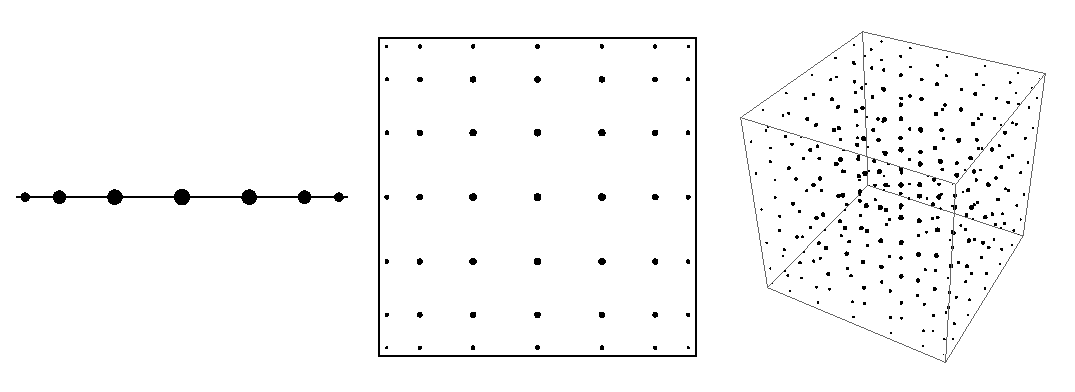
\includegraphics[height=0.25\textheight]{tensorproduct_quadrature.eps}
		\caption{St"utzstellen eines 1D 7--Punkt--Gauss--Legendre--Verfahrens und entsprechender Tensor--Produkt--Verfahren f"ur 2 bzw. 3 Dimensionen. Die Gewichte der St"utzstellen sind durch ihre Gr"o"se kenntlich gemacht.}
		\label{fig:tensorproduct}
	\end{figure}
	
	\subsubsection{einfache Monte--Carlo--Integration}
	Bei der Monte--Carlo--Integration ziehen wir $N$ zuf"allige, gem"a"s einer Wahrscheinlichkeitsdichte $p$ verteilte St"utzstellen $[X_i|i\in\{1,\dots,N\}]$ in $\Omega$ und sch"atzen dann den Wert des Integrals (\ref{eq:integration_problem}) mit
	\begin{equation}
		{\tilde I}_d^{\,\text{MC}}=\frac{1}{N}\sum_{i=0}^{N-1} \frac{f(X_i)}{p(X_i)}
		\label{eq:mc_integral}
	\end{equation}
	ab. Im Falle unseres $d$--dimensionalen Einheitsw"urfels $\Omega=[0,1]^d$ k"onnen wir besipielsweise jede St"utzstelle aus $d$ gleichf"ormig auf dem Einheitsintervall $[0,1]$ verteilten Zufallszahlen $U_i$ durch einfache Tupelbildung
	$$X_i:=(U_{d i},\dots,U_{d(i+1)-1})$$
	gewinnen. Von der Erwartungstreue des Sch"atzers (\ref{eq:mc_integral}) f"ur unser Integral (\ref{eq:integration_problem}) k"onnen wir uns mit \citep[][2.4]{Veach:1997p9136}
	\begin{align*}
		E[{\tilde I}_d^{\,\text{MC}}] &=E\left[\frac{1}{N}\sum_{i=0}^{N-1}\frac{f(X_i)}{p(X_i)}\right] \\
			&= \frac{1}{N}\sum_{i=0}^{N-1}E\left[\frac{f(X_i)}{p(X_i)}\right] \\
			&= \frac{1}{N}\sum_{i=0}^{N-1}\int_\Omega \frac{f(X_i)}{p(X_i)}p(X_i)\,d\mu(x) \\
			&= \int_\Omega f(x)\,d\mu(x)\\
			&= I
	\end{align*}
	leicht "uberzeugen.
	
	\subsubsection{Vergleich von Tensor--Produkt--Verfahren und einfacher Monte--Carlo--Integration}\label{subsec:integrationsproblem_comparison}
	Wir wollen nun die Konvergenzraten der Tensor--Produkt--Verfahren mit der Konvergenzrate des einfachen Monte--Carlo--Sch"atzers (\ref{eq:mc_integral}) vergleichen. Zur Konstruktion eines Vertreters der Tensor--Produkt--Verfahren verwenden wir beispielhaft das Newton--Cotes--Verfahren. In \citep[][3.1.4]{Stoer:2005p10586} wird als Absch"atzung f"ur den Fehler eines Verfahrens $p$--ter Ordnung (d.h. ein Verfahren, das alle Polynome bis zum Grad $p$ exakt integriert) und Schrittweite $h(\approx\frac{b-a}{N}=\mathcal{O}(N^{-1}))$ der St"utzstellen
	\begin{equation}
		\int_a^b P_n(x)-f(x)dx=h^{p+1}K f^{(p)}(\xi),\quad\xi\in(a,b)
		\label{eq:quadrature_error}
	\end{equation}
	angegeben, wobei $n$ die Anzahl der St"utzstellen, $P_n$ das Interpolationspolynom f"ur die St"utzstellen und K eine Konstante ist. Gauss--Legendre--Verfahren sind von der Ordnung $2n-1$, d.h. die Konvergenzrate dieser $n$--Punkt--Formel ist demnach von der Gr"o"senordnung $\mathcal{O}(h^{2n})=\mathcal{O}(N^{-2n})$.\footnote{$N$ bezeichnet die Anzahl der St"utzstellen f"ur das gesamte Integrationsintervall. Der Sch"atzwert f"ur das Integral wird dann durch $\frac{N}{n}$--maliges Anwenden der $n$--Punkt--Formel berechnet}
	Durch Bildund der entsprechenden $d$--dimensionalen Tensor--Produkt--Regel "andert sich die Konvergenzrate in Bezug auf die Schrittweite $h$ nicht. Da unsere $N$ St"utzstellen sich nun aber auf ein $d$--dimensionales Gitter verteilen, teilt sich das Volumen unseres $d$--dimensionalen Einheitsw"urfels in $N$ W"urfel mit einem Volumen von jeweils $h^d$ auf, d.h. f"ur die Schrittweite folgt
	$$\mathcal{O}(1)=V=N h^d \Rightarrow h=\mathcal{O}\left(\left(\frac{1}{N}\right)^{1/d}\right)=\mathcal{O}\left(N^{-1/d}\right)$$	
	und damit f"ur die Konvergenzrate in Bezug auf die Gesamtst"utzstellenzahl
	$$\mathcal{O}(h^{2n})=\mathcal{O}(N^{-2n/d}).$$
	Dies bedeutet, da"s Tensor--Produktverfahren mit steigender Dimension des Integrationsgebietes an Effizienz verlieren. Bei hochdimensionalen Problemen kann dies kaum durch Verfahren h"oherer Ordnung ausgeglichen werden, da Verfahren h"oherer Ordnung, wie oben in (\ref{eq:quadrature_error}) zu sehen auch gr"o"sere Anforderungen an die Glattheit der Funktion stellen. Ausserdem kann die exponentiell steigende Anzahl aller $N \geq n^d$ mindestens n"otigen Funktionsaufrufe zu einem Problem werden. Der Effekt wird bei steigender Dimension und Ordnung des Verfahrens nur noch schlimmer, was ein Ausgleichen der schlechteren Konvergenzrate bei h"oheren Dimensionen durch Erh"ohen der Ordnung des Verfahrens schnell praktisch unm"oglich werden l"asst. Dies wird h"aufig als {\em Curse~of~Dimensionality} (Fluch der Dimensionalit"at) bezeichnet.
	
	Bei der Monte--Carlo--Integration k"onnen wir die Konvergenzrate anhand der Varianz unseres Monte--Carlo--Sch"atzers (\ref{eq:mc_integral}) bestimmen \citep[][2.4.1]{Veach:1997p9136}. Nennen wir der "Ubersicht wegen
	$$Y_i=\frac{f(X_i)}{p(X_i)}$$
	und den MC--Sch"atzer mit $N$ gezogenenen Werten
	$$F_N=\frac{1}{N}\sum_{i=0}^{N-1} Y_i.$$
	Dann gilt f"ur die Varianz eines beliebigen Samples
	\begin{equation}
		V[Y_i]=E[(Y_i-E[Y_i])^2]=E[Y_i^2]-E[Y_i]^2=\int_\Omega \frac{f(x)^2}{p(x)}d\mu(x)-I^2.
		\label{eq:mc_variance}
	\end{equation}
	Da die Werte unabh"angig gezogen sind gilt f"ur die Varianz des Sch"atzer mit $N$ Werten
	$$V[F_N]=V\left[\frac{1}{N}\sum_{i=0}^{N-1}Y_i\right]=\frac{1}{N^2}V\left[\sum_{i=0}^{N-1}Y_i\right]=\frac{1}{N^2}\sum_{i=0}^{N-1}V[Y_i]=\frac{1}{N}V[Y_i],$$
	d.h. die Varianz des Sch"atzers sinkt invers mit der Anzahl $N$ an gezogenen Werten. Daraus folgt sofort die Standardabweichung
	$$\sigma[F_N]=\frac{1}{\sqrt{N}}\sigma[Y_i],$$
	was einer Konvergenzrate von $\mathcal{O}(N^{-1/2})$ entspricht. Die Konvergenzrate des Monte--Carlo--Sch"atzers ist im Gegensatz zur Konvergenzrate der Tensor--Produkt--Verfahren also unabh"angig von der Dimension des Integrationsgebietes, d.h. das Verfahren leidet {\em nicht} unter dem {\em Curse~of~Dimensionality}! Ausserdem mussten wir nirgendwo Bedingungen an die Glattheit der Funktion stellen, was bei Funktionen mit Diskontinuit"aten von Vorteil ist.
	
	Zusammenfassend k"onnen wir also feststellen, da"s Monte--Carlo--Integration bei hochdimensionalen Integrationsproblemen und Funktionen mit Diskontinuit"aten klar gegen"uber klassischen Tensor--Produktverfahren vorzuziehen ist. F"ur niedrigdimensionale ($d\lessapprox 7$) Gebiete mit glatten Integranden sind die klassischen Methoden hingegen besser geeignet.
	
	
	\subsection{Importance--Sampling}
	Wir sind bei unserem MC--Sch"atzer (\ref{eq:mc_integral}) nicht darauf beschr"ankt eine gleich\-f"or\-mi\-ge Wahrscheinlichkeitsdichte $p$ zu w"ahlen. Es kann sogar die Effizienz des Verfahrens betr"achtlich verbessern, wenn wir eine geeignete Wahrscheinlichkeitsdichte $p$ w"ahlen. Schauen wir uns daher die Formel (\ref{eq:mc_variance}) f"ur die Varianz nochmal an, da"s es zu minimieren gilt, um zu verstehen, was ``geeignet'' bedeutet. Nimmt die Wahrscheinlichkeitsdichte beispielsweise die ideale Form
	\begin{equation}
		p(x)=\frac{|f(x)|}{\int_\Omega |f(z)|d\mu(z)}
		\label{eq:ideal_importance_pdf}
	\end{equation}
	an, kann man mit der {\em Jensenschen~Ungleichung} zeigen, da"s dann das Integral in (\ref{eq:mc_variance}) und damit die Varianz insgesamt minimal wird. Nimmt $f$ keine negativen Werte an, verschwindet die Varianz dieses Sch"atzers sogar, da in (\ref{eq:mc_integral}) dann nur noch "uber die konstante L"osung (in Form der Normierungskonstanten) gemittelt wird. Wenn wir das Normierungs--Integral im Nenner von (\ref{eq:ideal_importance_pdf}) l"osen k"onnten, w"are allerdings auch die urspr"ungliche Integration (\ref{eq:integration_problem}) kein Problem! Daher suchen wir in der Praxis nach einem $p$, das m"oglichst "ahnlich zu $|f|$ und gleichzeitig normierbar ist.
	
	
	\subsection{Monte--Carlo--Markov--Chain--Verfahren}
	Bisher sind wir bei unserem Monte--Carlo--Sch"atzer (\ref{eq:mc_integral}) von einer zugrundeliegenden Stichprobe aus $N$ unabh"angigen und identisch gem"a"s $p$ verteilten St"utzstellen ausgegangen, deren zugeh"rige Funktionswerte gemittelt als Sch"atzer f"ur den Wert des Integrals (\ref{eq:integration_problem}) dienen. Wenn wir aber unsere Funktionswerte in jedem Fall mitteln, dann ist die Unabh"angigkeit der gezogenen St"utzstellen nicht relevant, da die Reihenfolge, in der sie gezogen werden, den Mittelwert nicht beeinflusst. Essentiell ist also lediglich, dass sie identisch gem"a"s $p$ verteilt sind.
	
	Diese Freiheit nutzen sogenannte Monte--Carlo--Markov--Chain--Verfahren (MCMC--Verfahren). Sie stellen ein Verfahren dar, um aus einem Zustandsraum $\Omega$ gem"a"s einer gegebenen Wahrscheinlichkeitsdichte $p$ verteilte Werte zu ziehen. Dies wird durch die Konstruktion eines Zufallspfads ({\em random~walk}) im Zustandsraum, dirigiert durch eine Markov--Kette, erreicht. Dabei mu"s sichergestellt werden, da"s die so erzeugten Werte auch gem"a"s $p$ verteilt sind und insbesondere jeder Punkt im Zustandsraum, auf dem $p$ nicht verschwindet, auch erreicht werden kann.
	
	Wie im n"achsten Abschnitt gezeigt wird, ist dies mit erstaunlich wenig Aufwand m"oglich. Die Kombination aus Vielseitigkeit, M"achtigkeit und Einfachheit hat MCMC--Verfahren in vielen Bereichen\footnote{Beispiele finden sich u.a. in der statistischen Physik, in der Finanzmathematik und zur Berechnung von A--posteriori--Wahrscheinlichkeiten in der Bayes'schen Statistik \citep{Geweke:1989p10465}, z.B. mit Anwendungen in der Bioinformatik und Medizin. Weitere interessante und ungew"ohnliche Anwendungen finden sich in \citep{Diaconis:2009p4122}} zu einem Hauptverfahrensbestandteil gemacht.
	
	
	\subsubsection{Metropolis--Hastings--Algorithmus}
	Unter den MCMC--Verfahren ist eines der bekanntesten der {\em Metropolis--Hastings--Algorithmus} (MH), der durch eine Arbeit in der statistischen Physik von \citet{Metropolis:1953p3364} in einer einfachen Form vorgestellt und sp"ater durch \citet{Hastings:1970p3387} verallgemeinert wurde.

	Beim MH--Algorithmus ziehen wir aus einem Zustandsraum $\Omega$ Elemente $x \in \Omega$ gem"a"s der (nicht notwendigerweise normierten!) Wahrscheinlichkeitsdichte $f : \Omega \rightarrow \mathbb{R}_{\geq 0}$. Die Elemente werden dabei mit einem Zufallspfad durch den Zustandsraum generiert. Wir ver"andern dazu den aktuellen Zustand $x$ nach einem frei w"ahlbaren Schema (im Folgenden Mutation genannt) in einen neuen Zustand $x'$.
	Dabei stellen wir folgende Bedingungen an eine Mutation:
	\begin{itemize}
		\item{wenn der "Ubergang vom Zustand $x$ nach $x'$ m"oglich ist, muss auch der "Ubergang zur"uck von $x'$ nach $x$ m"oglich sein}
		\item{es muss jeder Zustand $x \in \Omega$ durch eine Kette von "Uberg"angen erreichbar sein (Ergodizit"at)}
		\item{Die "Ubergangswahrscheinlichkeit $T(x'|x)$ durch unser Mutations--Schema von Zustand $x$ zum Zustand $x'$ zu kommen muss f"ur gegebenes $x$ und $x'$ berechenbar sein}
	\end{itemize}
	Mutationen sind also etwas formaler formuliert bedingte Wahrscheinlichkeitsverteilungen, die durch das Herkunftselements parametrisiert sind, nicht normiert sein m"ussen und f"ur die
	$$\forall x,x'\in\Omega : \quad T(x'|x)>0 \Leftrightarrow T(x|x')>0$$
	wahr ist.
	
	\paragraph{Detailed Balance:}
	Da die Mutation, mit der wir den neuen Zustand generieren, nichts mit der Wahrscheinlichkeitsdichte $f$ zu tun haben mu"s, brauchen wir eine M"oglichkeit die Verteilung der Zust"ande gem"a"s $f$ sicherzustellen.
	Betrachten wir eine gro"se Zahl von gleichartigen aber unabh"angigen Markov--Ketten, die alle mit einer gewissen Wahrscheinlichkeit $p(x'|x)$ vom Zustand $x$ in den Zustand $x'$ "ubergehen, dann ist eine M"oglichkeit eine station"are Zustandsdichte $f$, gemittelt "uber die aktuellen Zust"ande aller Markov--Ketten, zu erreichen, zu verlangen, da"s
	\begin{equation}
		\forall x,x' \in \Omega :\quad f(x)p(x'|x) = f(x')p(x|x')
		\label{eq:dynamic_equlibrium}
	\end{equation}
	({\em =Detailed Balance}) gilt, d.h. da"s die "Ubergangsraten zwischen zwei beliebigen Zust"anden sich im dynamischen Gleichgewicht befinden.
	Da $T$ die "Ubergangswahrscheinlichkeiten aber schon festlegt, behalten wir uns das Recht vor, einen durch Ziehen aus $T$ vorgeschlagenen Zustands"ubergang nur mit der Wahrscheinlichkeit $a(x'|x)$ anzunehmen und ansonsten abzulehnen,	um {\em Detailed Balance} sicherstellen zu k"onnen:
	\begin{equation}
		p(x'|x) = T(x'|x)a(x'|x)
		\label{eq:acceptance_prob_intro}
	\end{equation}
	\begin{equation}
		(\ref{eq:dynamic_equlibrium}) \stackrel{(\ref{eq:acceptance_prob_intro})}{\Longrightarrow}
		\forall x,x' \in \Omega :\quad f(x)T(x'|x)a(x'|x) = f(x')T(x|x')a(x|x')
		\label{eq:detailedbalance}
	\end{equation}
	Dies l"asst noch immer verschiedene M"oglichkeiten zu, die Akzeptanzwahrscheinlichkeit zu bestimmen. Eine effiziente und dadurch beliebte Wahl ist dabei Folgende: ist $f(x')>f(x)$ nehmen wir den neuen Zustand auf jeden Fall an, ansonsten mit der Wahrscheinlichkeit $(f(x')T(x|x'))/(f(x)T(x'|x))$. Dies l"asst sich zusammenfassen zu
	\begin{equation}
		a(x'|x)=\text{min}\left(1,\frac{f(x')T(x|x')}{f(x)T(x'|x)}\right)
		\label{eq:acceptanceratio}
	\end{equation}
	
	
	\paragraph{Pseudocode:}
	In Pseudocode sieht der Algorithmus dann wie folgt aus:
	\begin{algorithmic}
		\STATE $x_1 \leftarrow$ Anfangszustand
		\FOR{$i=1$ to $N$}
			\STATE ziehe $x'$ gem"a"s $T(x'|x_i)$
			\STATE $a(x'|x_i) \leftarrow \text{min}\left(1, \frac{f(x')T(x|x')}{f(x)T(x'|x)}\right)$
			\STATE $u\leftarrow$ Zufallszahl aus $[0,1]$
			\IF{$u < a(x'|x_i)$}	\STATE $x_{i+1}=x'$
			\ELSE	\STATE $x_{i+1}=x_i$
			\ENDIF
	  \ENDFOR
	\end{algorithmic}
	Als Ergebnis erhalten wir eine Liste von Samples, die gem"a"s $f$ verteilt sind. Die Samples sind allerdings nicht unabh"angig, sondern im Gegenteil h"aufig hochkorreliert. Wenn wir nur an statistischen Kenngr"o"sen wie dem Mittelwert oder der Varianz einer Stichprobe interessiert sind ist die Korrelation aber irrelevant und stellt somit f"ur uns kein Problem dar. Die Tatsache, da"s die Normierung von $f$ f"ur die Funktion des Verfahrens nicht notwendig ist, bedeutet allerdings auch, da"s wir uns bei Bedarf eine Normierung auf andere Weise beschaffen m"ussen.
	
	
	\subsubsection{Generalisierter Metropolis--Hastings--Algorithmus}
	TODO: Robuste MH--Variante

	\section{Monte--Carlo--Strahlungstransport}
	\subsection{Pfadgenerierung}
	\subsubsection{Raycasting}
	\subsubsection{Distanzsampler}
	TODO: uniform depth sampler, uniform attenuation sampler, enforced uniform attenuation sampler
	
	TODO: Pfadgenerierung, Sch"atzer

	
	\section{Testf"alle und Resultate}
	\subsection{Homogene streuende Kugel}
	TODO: Motivation? tau=0.01,1,10
	\subsubsection{analytische L"osung}
	\subsubsection{Resultate}
	TODO: Vergleich mit analytischer L"osung und MC3D (Ergebnis+Geschwindigkeit)
	\subsection{Einfaches Scheibenmodell}
	\subsubsection{Resultate}
	TODO: Vergleich mit MC3D (Ergebnis und Geschwindigkeit)
	\subsection{Einordnung der Resultate}
	TODO: Gesamtvergleich zwischen MC3D und PIRaTE
	
	\section{Programmbeschreibung}
	TODO: Programmbeschreibung in Worten bzw. Pseudocode, Modulbeschreibung, Details in evtl. Anhang auslagern.
	
	\section{Zusammenfassung und Ausblick}
	TODO: Ausblick: Normierung, physikalisch relevante Streuphasenfunktionen, polychromatische Bilder/SEDs

	\bibliographystyle{chicago}
	\bibliography{bibliography}
\end{document}